% Create a Table of Contents in Beamer
\documentclass[10pt,t]{beamer}
% Theme choice:
\usetheme{Singapore}
\useoutertheme{sidebar}
\usecolortheme{seahorse}
\setbeamercolor{titlelike}{bg=white}
\setbeamercolor{frametitle}{bg=white}
%\setbeamertemplate{frametitle}[default][left]
\setbeamertemplate{navigation symbols}{}
\setbeamertemplate{footline}{\begin{flushright}\large \insertframenumber\end{flushright}}

\usepackage{graphicx}
\usepackage{amsmath}
\usepackage{amsfonts}
\usepackage{amssymb}
\usepackage{amsthm}
\usepackage{verbatim}

% Title page details: 
\title{Chapter 0: Review} 
\author{Nina Galanter}
\date{March 29, 2023}



\begin{document}
	
	
	\begin{frame}{Announcements and Reminders}
		
		\begin{itemize}
			\item Everyone will get credit for the first pollev 
			\medskip
			\item Slight change to quiz timing: they will be graded by noon Wednesday and revisions due by noon Friday
			\medskip
			\item Complete the background quiz by the end of today
			\medskip
			\item Fill out the office hour poll (in the first announcement) ASAP
			\medskip
			\item Remember to turn in discussion section activity
			\medskip
			\item First homework will be released tomorrow
		\end{itemize}
		
	\end{frame}
	
	% Title page frame
	\begin{frame}
	\titlepage 
	
	\centering
	\textbf{pollev.com/ninag}
\end{frame}




\begin{frame}{Learning objectives}
By the end of Chapter 0, you should be able to:
\medskip
\begin{itemize}
	\item Identify and describe common study designs
	\item Classify variables according to their type (e.g., binary)
	\item Use numerical and graphical tools to summarize data
	\item Explain features of and calculate probabilities using important probability distributions (Normal, $t$) 
	\item Define a sampling distribution
	\item Understand the importance of the Central Limit Theorem for statistical inference
	\item Construct and interpret confidence intervals
	\item Formulate null and alternative hypotheses
	\item Choose, implement, and interpret hypothesis tests
\end{itemize}
\end{frame}

% Outline frame
\begin{frame}{Outline}
\tableofcontents
\end{frame}

\AtBeginSection[ ]
{
\begin{frame}{Outline}
\tableofcontents[currentsection]
\end{frame}
}

% Presentation structure
\section{Study Design}

\begin{frame}{Study Design}
\textbf{How you collect data impacts what questions you can (cannot) answer, what statistical methods you can (cannot) use, and what conclusions you can (cannot) draw.} \\~\

\textcolor{blue}{Extreme Example:} Suppose I'm interested in understanding public opinion about biostatistics. I randomly select an individual from our class and ask if they like biostatistics.

\begin{itemize}
	\item What questions can I answer using these data?
	\item What statistical methods can I use to analyze these data?
	\item What conclusions can I draw using these data?
\end{itemize}
\end{frame}

\begin{frame}{Study Design: language}
	A quick reminder about language:
	
	\vspace{0.3cm}
	
	\begin{itemize}
		\item \textcolor{blue}{Exposure}: an explanatory variable that may be associated with (or causally related to) the outcome of interest. This is not always an exposure in the colloquial sense, such as someone being ``exposed" to a disease!
		\item \textcolor{blue}{Outcome}: the variable we are primarily interested in measuring or predicting
	\end{itemize}
\vspace{0.3cm}
Examples: 
\vspace{0.3cm}
\begin{itemize}
	\item Vaccination (exposure) and positive COVID test result (outcome)
	\item Tutoring (exposure) and final course grade (outcome)
	\item Age (exposure) and cancer occurrence (outcome)
\end{itemize}
\end{frame}

\begin{frame}{Experimental vs. Observational Studies}

\textcolor{blue}{Experimental:} exposure/treatment is \textbf{controlled} by the researcher (e.g., randomly assign people to drug or placebo)
\begin{itemize}
	\item Randomized controlled trial 
\end{itemize}

\vspace{0.3cm}

\textcolor{blue}{Observational:} exposure/treatment is \textbf{not controlled} by the researcher (e.g., we look at a group of people and \textbf{observe} who smokes and who doesn't smoke)
\begin{itemize}
	\item Cross-sectional study
	\item Cohort study
	\item Case-control study
\end{itemize}
\end{frame}
	
	
\begin{frame}{Experimental vs. Observational Studies}
In \textbf{experimental} studies, we can talk about \color{blue} \textbf{causation}\color{black}. In \textbf{observational} studies we  talk instead about \color{blue} \textbf{association} \color{black}(because we worry about \color{blue} \textbf{confounding}\color{black}). \\

\vspace{0.3cm}

% we'll come back to this when we talk about interpreting results
A \textbf{\textcolor{blue}{confounder}} is a variable that is \textbf{causally related to} our outcome and also \textbf{associated with} the exposure in our sample.  \\

\vspace{0.3cm}

\begin{itemize}
	\item[] \textbf{Example:} suppose we're interested in the relationship between smoking and lung function in kids. We know that age is causally associated with lung function: as children grow and develop, their lung function improves. If age is also associated with smoking in our sample (e.g., if older kids are more likely to smoke), then age is a confounder.
\end{itemize} 

\vspace{0.3cm}

\small \textbf{Much more on the topic of confounding to come...} 
\end{frame}

\subsection{Experimental studies}

\begin{frame}{Randomized controlled trial}
Description:
\begin{itemize}
	\item Take a sample from the population and \textbf{randomly assign} individuals to either treatment (\textbf{exposed}) or control/placebo (\textbf{unexposed})
	\item Follow individuals to observe a specific outcome (e.g., death yes/no, disease yes/no, time to death, change in cholesterol level, \dots)
\end{itemize}
\end{frame}

\begin{frame}{Randomized controlled trial}
Description:
\begin{itemize}
	\item Take a sample from the population and \textbf{randomly assign} individuals to either treatment (\textbf{exposed}) or control/placebo (\textbf{unexposed})
	\item Follow individuals to observe a specific outcome (e.g., death yes/no, disease yes/no, time to death, change in cholesterol level, \dots)
\end{itemize}
Pros:
\begin{itemize}
	\item With a large enough sample, no confounding
	\item Gold standard for establishing causality
\end{itemize}
\end{frame}

\begin{frame}{Randomized controlled trial}
Description:
\begin{itemize}
	\item Take a sample from the population and \textbf{randomly assign} individuals to either treatment (\textbf{exposed}) or control/placebo (\textbf{unexposed})
	\item Follow individuals to observe a specific outcome (e.g., death yes/no, disease yes/no, time to death, change in cholesterol level, \dots)
\end{itemize}
Pros:
\begin{itemize}
	\item With a large enough sample, no confounding
	\item Gold standard for establishing causality
\end{itemize}
Cons:
\begin{itemize}
	\item Often very expensive
	\item Not always possible or ethical to randomize individuals
	\begin{itemize}
		\item Cannot randomly assign someone to a specific air pollution level, genetic variant, etc.
		\item Unethical to randomly assign harmful exposures (e.g., smoking)
	\end{itemize}
\end{itemize}
\end{frame}

\begin{frame}[c]{Randomized controlled trial}
Examples: 

\vspace{0.3cm}

\begin{itemize}
	\item \href{https://jamanetwork.com/journals/jama/article-abstract/2613159}{\color{cyan} Effect of Vitamin D and Calcium Supplementation on Cancer Incidence in Older Women}
	\item \href{http://stroke.ahajournals.org/content/36/8/1764.short}{\color{cyan} Daily Functioning and Quality of Life in a Randomized Controlled Trial of Therapeutic Exercise for Subacute Stroke Survivors}
\end{itemize}

\end{frame}


\subsection{Observational studies}

\begin{frame}{Cross-sectional study}
Description:
\begin{itemize}
	\item Randomly sample individuals, record their exposure and outcome at a \textbf{single time point/interval} (no follow-up)
\end{itemize}
\end{frame}

\begin{frame}{Cross-sectional study}
Description:
\begin{itemize}
	\item Randomly sample individuals, record their exposure and outcome at a \textbf{single time point/interval} (no follow-up)
\end{itemize}
\medskip
Pros:
\begin{itemize}
	\item Relatively cheap and easy
	\item Can study multiple outcomes and exposures
\end{itemize}
\end{frame}

\begin{frame}{Cross-sectional study}
Description:
\begin{itemize}
	\item Randomly sample individuals, record their exposure and outcome at a \textbf{single time point/interval} (no follow-up)
\end{itemize}
\medskip
Pros:
\begin{itemize}
	\item Relatively cheap and easy
	\item Can study multiple outcomes and exposures
\end{itemize}
\medskip
Cons:
\begin{itemize}
	\item Inefficient for rare exposure and disease 
	\item Time sequence of exposure and outcome (i.e. which came first) is not always clear
	\item Potential confounding (so no conclusions about causality)
\end{itemize}
\end{frame}

\begin{frame}[c]{Cross-sectional study}
Examples:
\vspace{0.3cm}

\begin{itemize}
	\item \href{http://ajph.aphapublications.org/doi/abs/10.2105/AJPH.78.10.1336}{\color{cyan} Job strain, work place social support, and cardiovascular disease in a random sample of the Swedish working population}
	\item \href{onlinelibrary.wiley.com/doi/10.1111/add.12623/full}{\color{cyan} Real-world effectiveness of e-cigarettes when used to aid smoking cessation}
\end{itemize}



\end{frame}

\begin{frame}{Cohort study}
Description:
\begin{itemize}
	\item Sample people \textbf{without the outcome of interest}, record their exposure, then \textbf{follow} them over time to observe the outcome
	\item Can be \textbf{prospective} (sample people in present time, then follow-up) or \textbf{restrospective} (sample people from a database collected in the past, and observe them through their time recorded in the database)
\end{itemize}
\end{frame}

\begin{frame}{Cohort study}
Description:
\begin{itemize}
	\item Sample people \textbf{without the outcome of interest}, record their exposure, then \textbf{follow} them over time to observe the outcome
	\item Can be \textbf{prospective} (sample people in present time, then follow-up) or \textbf{restrospective} (sample people from a database collected in the past, and observe them through their time recorded in the database)
\end{itemize}
Pros:
\begin{itemize}
	\item Time sequence is known (exposure came first)
	\item Can study multiple outcomes 
\end{itemize}
\end{frame}

\begin{frame}{Cohort study}
Description:
\begin{itemize}
	\item Sample people \textbf{without the outcome of interest}, record their exposure, then \textbf{follow} them over time to observe the outcome
	\item Can be \textbf{prospective} (sample people in present time, then follow-up) or \textbf{restrospective} (sample people from a database collected in the past, and observe them through their time recorded in the database)
\end{itemize}
Pros:
\begin{itemize}
	\item Time sequence is known (exposure came first)
	\item Can study multiple outcomes 
\end{itemize}
Cons:
\begin{itemize}
	\item Inefficient for rare outcomes
	\item Prospective cohort studies are often expensive and time-consuming to follow people, and people may drop out/be lost to follow up
	\item Potential confounding (so no conclusions about causality)
\end{itemize}
\end{frame}

\begin{frame}[c]{Cohort study}
Examples:
\vspace{0.3cm}

\begin{itemize}
	\item \href{https://www.medicalnewstoday.com/articles/316619.php}{\color{cyan} Drinking tea could help stave off cognitive decline}
	\item \href{https://www.medicalnewstoday.com/articles/316565.php}{\color{cyan} Birth control pills may protect against some cancers for decades}
\end{itemize}



\end{frame}

\begin{frame}{Case-control study}
	\vspace{-5 mm}
Description:
\begin{itemize}
	\item Sample individuals \textbf{based on the outcome} (some with, some without), look back in time (usually) for exposure
\end{itemize}
\end{frame}

\begin{frame}{Case-control study}
	\vspace{-5 mm}
Description:
\begin{itemize}
	\item Sample individuals \textbf{based on the outcome} (some with, some without), look back in time (usually) for exposure
\end{itemize}
Pros:
\begin{itemize}
	\item Efficient for rare diseases
	\item Cheaper and faster than cohort studies
	\item Can study multiple exposures
\end{itemize}
\end{frame}

\begin{frame}{Case-control study}
	\vspace{-5 mm}
Description:
\begin{itemize}
	\item Sample individuals \textbf{based on the outcome} (some with, some without), look back in time (usually) for exposure
\end{itemize}
Pros:
\begin{itemize}
	\item Efficient for rare diseases
	\item Cheaper and faster than cohort studies
	\item Can study multiple exposures
\end{itemize}
Cons:
\begin{itemize}
	\item May not know time sequence of disease and exposure
	\item Cannot estimate relative risk or outcome prevalence*
\begin{itemize}
\item \textcolor{blue}{Sample outcome prevalence chosen/driven by researchers}
\item \textcolor{blue}{Sample prevalence and risk can't be used to estimate population prevalence and risk}
	\end{itemize}	
	\item Potential confounding (so no conclusions about causality)
\end{itemize}
\medskip
*Generally, odds ratio approximates risk ratio for "rare" outcomes
\end{frame}



\begin{frame}[c]{Case-control study}
Examples:
\vspace{0.3cm}

\begin{itemize}
	\item \href{https://www.sciencedirect.com/science/article/pii/S0140673605676635}{\color{cyan}Obesity and the risk of myocardial infarction in 27,000 participants from 52 countries}
	\item \href{http://www.nejm.org/doi/full/10.1056/NEJMoa065497\#t=article}{\color{cyan}Case control study of human papillomavirus and oropharyngeal cancer}
\end{itemize}

\end{frame}

\begin{frame}{Study design: Practice}
You read \href{https://jamanetwork.com/journals/jamaoncology/fullarticle/2569059?resultClick=24}{\color{cyan} this article} (from 2017), interested in the association between androgen deprivation therapy (ADT), a treatment for prostate cancer, and risk of dementia. \\~\

From the article: \textbf{In this... study, a text-processing method was used to analyze electronic medical record data from... 1994 to 2013. We identified 9455 individuals with prostate cancer who were 18 years or older at diagnosis with data recorded in the electronic health record and follow-up after diagnosis. We tested the effect of ADT on the risk of dementia.}

\vspace{0.3cm}

\begin{itemize}
	\item What kind of study design is this? \textcolor{violet}{POLLEV Question}
	\item Why do you think they chose this design? % cheap, can't randomly assign ADT
	\item What are potential limitations of this study design?
\end{itemize}


\end{frame}

%\begin{frame}{Study design: Practice}
%\begin{itemize}
%	\item What kind of study design is this?
%	\medskip
%	\begin{itemize}
%		\item[]  \color{blue} Cohort study (retrospective)
%	\end{itemize}
%\medskip
%	\item Why do you think they chose this design? % cheap, can't randomly assign ADT
%		\medskip
%	\begin{itemize}
%		\item \color{blue} Randomized controlled trials impossible, since you can't (and wouldn't) randomly assign prostate cancer
%		\smallskip
%		\item \color{blue} Dementia is not particularly rare, and they likely wanted to make statements about relative risks, so case-control studies are out
%		\smallskip
%		\item  Cross-sectional studies wouldn't necessarily allow the researchers to determine if dementia came before or after ADT. It may also be difficult to ask individuals with dementia about their history with ADT
%		\smallskip
%		\item Retrospective cohort studies are cheap, and easily allow the researchers to know whether or not ADT came before dementia \textbf{and} how long of a time there was between ADT and dementia, which may be of interest
%	\end{itemize}
%\end{itemize}
%\end{frame}
%
%\begin{frame}{Study design: Practice}
%\begin{itemize}
%	\item What are potential limitations of this study design?
%	\medskip
%	\begin{itemize}
%		\item[] \color{blue} Potential confounding: cannot conclude that ADT causes / does not cause dementia
%	\end{itemize}
%\end{itemize}
%\end{frame}

\begin{frame}{\textcolor{violet}{POLLEV} Study design: Practice}
Suppose you are interested in determining whether or not tobacco smoking increases the risk of schizophrenia. The prevalence of schizophrenia in the general population, either globally or in the US, is estimated to be under 1\%. Which study design would be most appropriate for answering your research question, and why?
\bigskip

\begin{itemize}
	\item Randomized clinical trial
	\item Cross-sectional study
	\item Cohort study
	\item Case-control study
\end{itemize}
\end{frame}

%\begin{frame}{\textcolor{violet}{POLLEV} Study design: Practice}
%Suppose you are interested in determining whether or not tobacco smoking increases the risk of schizophrenia. The prevalence of schizophrenia in the general population, either globally or in the US, is estimated to be under 1\%. Which study design would be most appropriate for answering your research question, and why?
%\bigskip
%
%\color{blue} Case-control study. 
%
%\bigskip
%
%\begin{itemize}
%	\item not ethical to randomize exposure to tobacco smoking so a clinical trial is out
%	\item We want to look at smoking as an exposure that comes before schizophrenia in time, so a cross-sectional study makes less sense
%	\item as schizophrenia is rare, a cohort study would need to be \textbf{very, very} large to get a reasonable number of people with the outcome 
%\end{itemize}


%\end{frame}

\begin{frame}{\textcolor{violet}{POLLEV} Study design: Practice}
	You are interested in studying the existence and extent of racial disparities in access to online patient portals for primary health care. Which study design would be most appropriate for answering your research question, and why?
	\bigskip
	
	\begin{itemize}
		\item Randomized clinical trial
		\item Cross-sectional study
		\item Cohort study
		\item Case-control study
	\end{itemize}
\end{frame}

%\begin{frame}{\textcolor{violet}{POLLEV} Study design: Practice}
%	You are interested in studying the existence and extent of disparities in access to online patient portals for primary health care based on self-identified race. Which study design would be most appropriate for answering your research question, and why?
%	\bigskip
%	
%	\textcolor{blue}{Cross-sectional study}
%	\bigskip
%	
%	\begin{itemize}
%		\item We aren't trying to determine a causal relationship
%		\item We are trying to look at the current point in time prevalence of access to patient portals
%	\end{itemize}
%\end{frame}

\begin{frame}[c]
\centering \huge Any Questions?
\end{frame}

\section{Summarizing data}


\begin{frame}{Motivating Dataset}
Throughout this chapter (and the next), we'll be exploring data containing a random sample of 2500 singleton births in King County in 2001. In 1989, Seattle and King County started a program called \href{https://kingcounty.gov/depts/health/child-teen-health/maternity-support-infant-case-management.aspx}{\textcolor{cyan}{First Steps}} which provides free pre-natal care to low-income, pregnant individuals. 

\vspace{0.3cm}

The goal of the program is to improve birth outcomes, including increased birthweights in King County. Low infant birthweight is one of the most important factors affecting neonatal mortality. 

\end{frame}

\begin{frame}{Motivating Dataset}
Variables in the dataset include:

\vspace{0.3cm}


\begin{itemize}
	\item Participation in First Steps (yes/no)
	\item Birth parent's age at time of birth (years)
	\item Marital status of birth parent (married yes/no)
	\item Child's gestational age at birth (weeks)
	\item Parity (number of children in family)
	\item Smoking during pregnancy (yes/no)
	\item Drinking during pregnancy (yes/no)
	\item And more!
\end{itemize}

\vspace{0.3cm} 

\textbf{We'll refer to this dataset as the \textcolor{blue}{births} dataset.} Available on the Canvas site as \color{blue} births.csv
\end{frame}

\subsection{Types of Variables}

\begin{frame}{Types of Variables}
\textbf{How you summarize/analyze data often depends on what type of data you've collected.}

\vspace{0.3cm}

The first step to summarizing/describing data is making sure you know what kind of data you have!

\end{frame}

\begin{frame}{Types of Variables}

\textcolor{blue}{Categorical:} 

\vspace{0.3cm}

\begin{itemize}
	\item \textbf{Nominal:} order has no meaning (e.g., country)
	\item \textbf{Ordinal:} order may be meaningful (e.g., level of education)
	\item \textbf{Binary:} two possible values; nominal or ordinal (e.g., presence of a genetic variant)
\end{itemize}

\vspace{0.3cm}

\textcolor{blue}{Quantitative:} 

\vspace{0.3cm}

\begin{itemize}
	\item \textbf{Discrete:} values are typically integers (e.g., number of people living with HIV)
	\item \textbf{Continuous:} values on a continuum (e.g., time)
\end{itemize}

\end{frame}

\begin{frame}{Types of Variables: Activity}

Sometimes determining variable type is complicated! Consider the following scenario:

\vspace{0.3cm}

We survey parents and record information on whether or not they have any children. 
\bigskip

We record each living child's age, and if any of their children have died, we record the child's age of death.
\bigskip

 Age at death is recorded monthly from age 0 months to 24 months, and yearly after that. 

\end{frame}

\begin{frame}{Types of Variables: Activity}

\vspace{-5 mm}

We survey parents and record information on whether or not they have any children. 
\medskip

We record each living child's age, and if any of their children have died, we record the child's age of death. 
\medskip

Age at death is recorded monthly from age 0 months to 24 months, and yearly after that. 
\medskip

We plot the number of children who died at each age recorded vs. age in months:

\vspace{0.3cm}

\centering 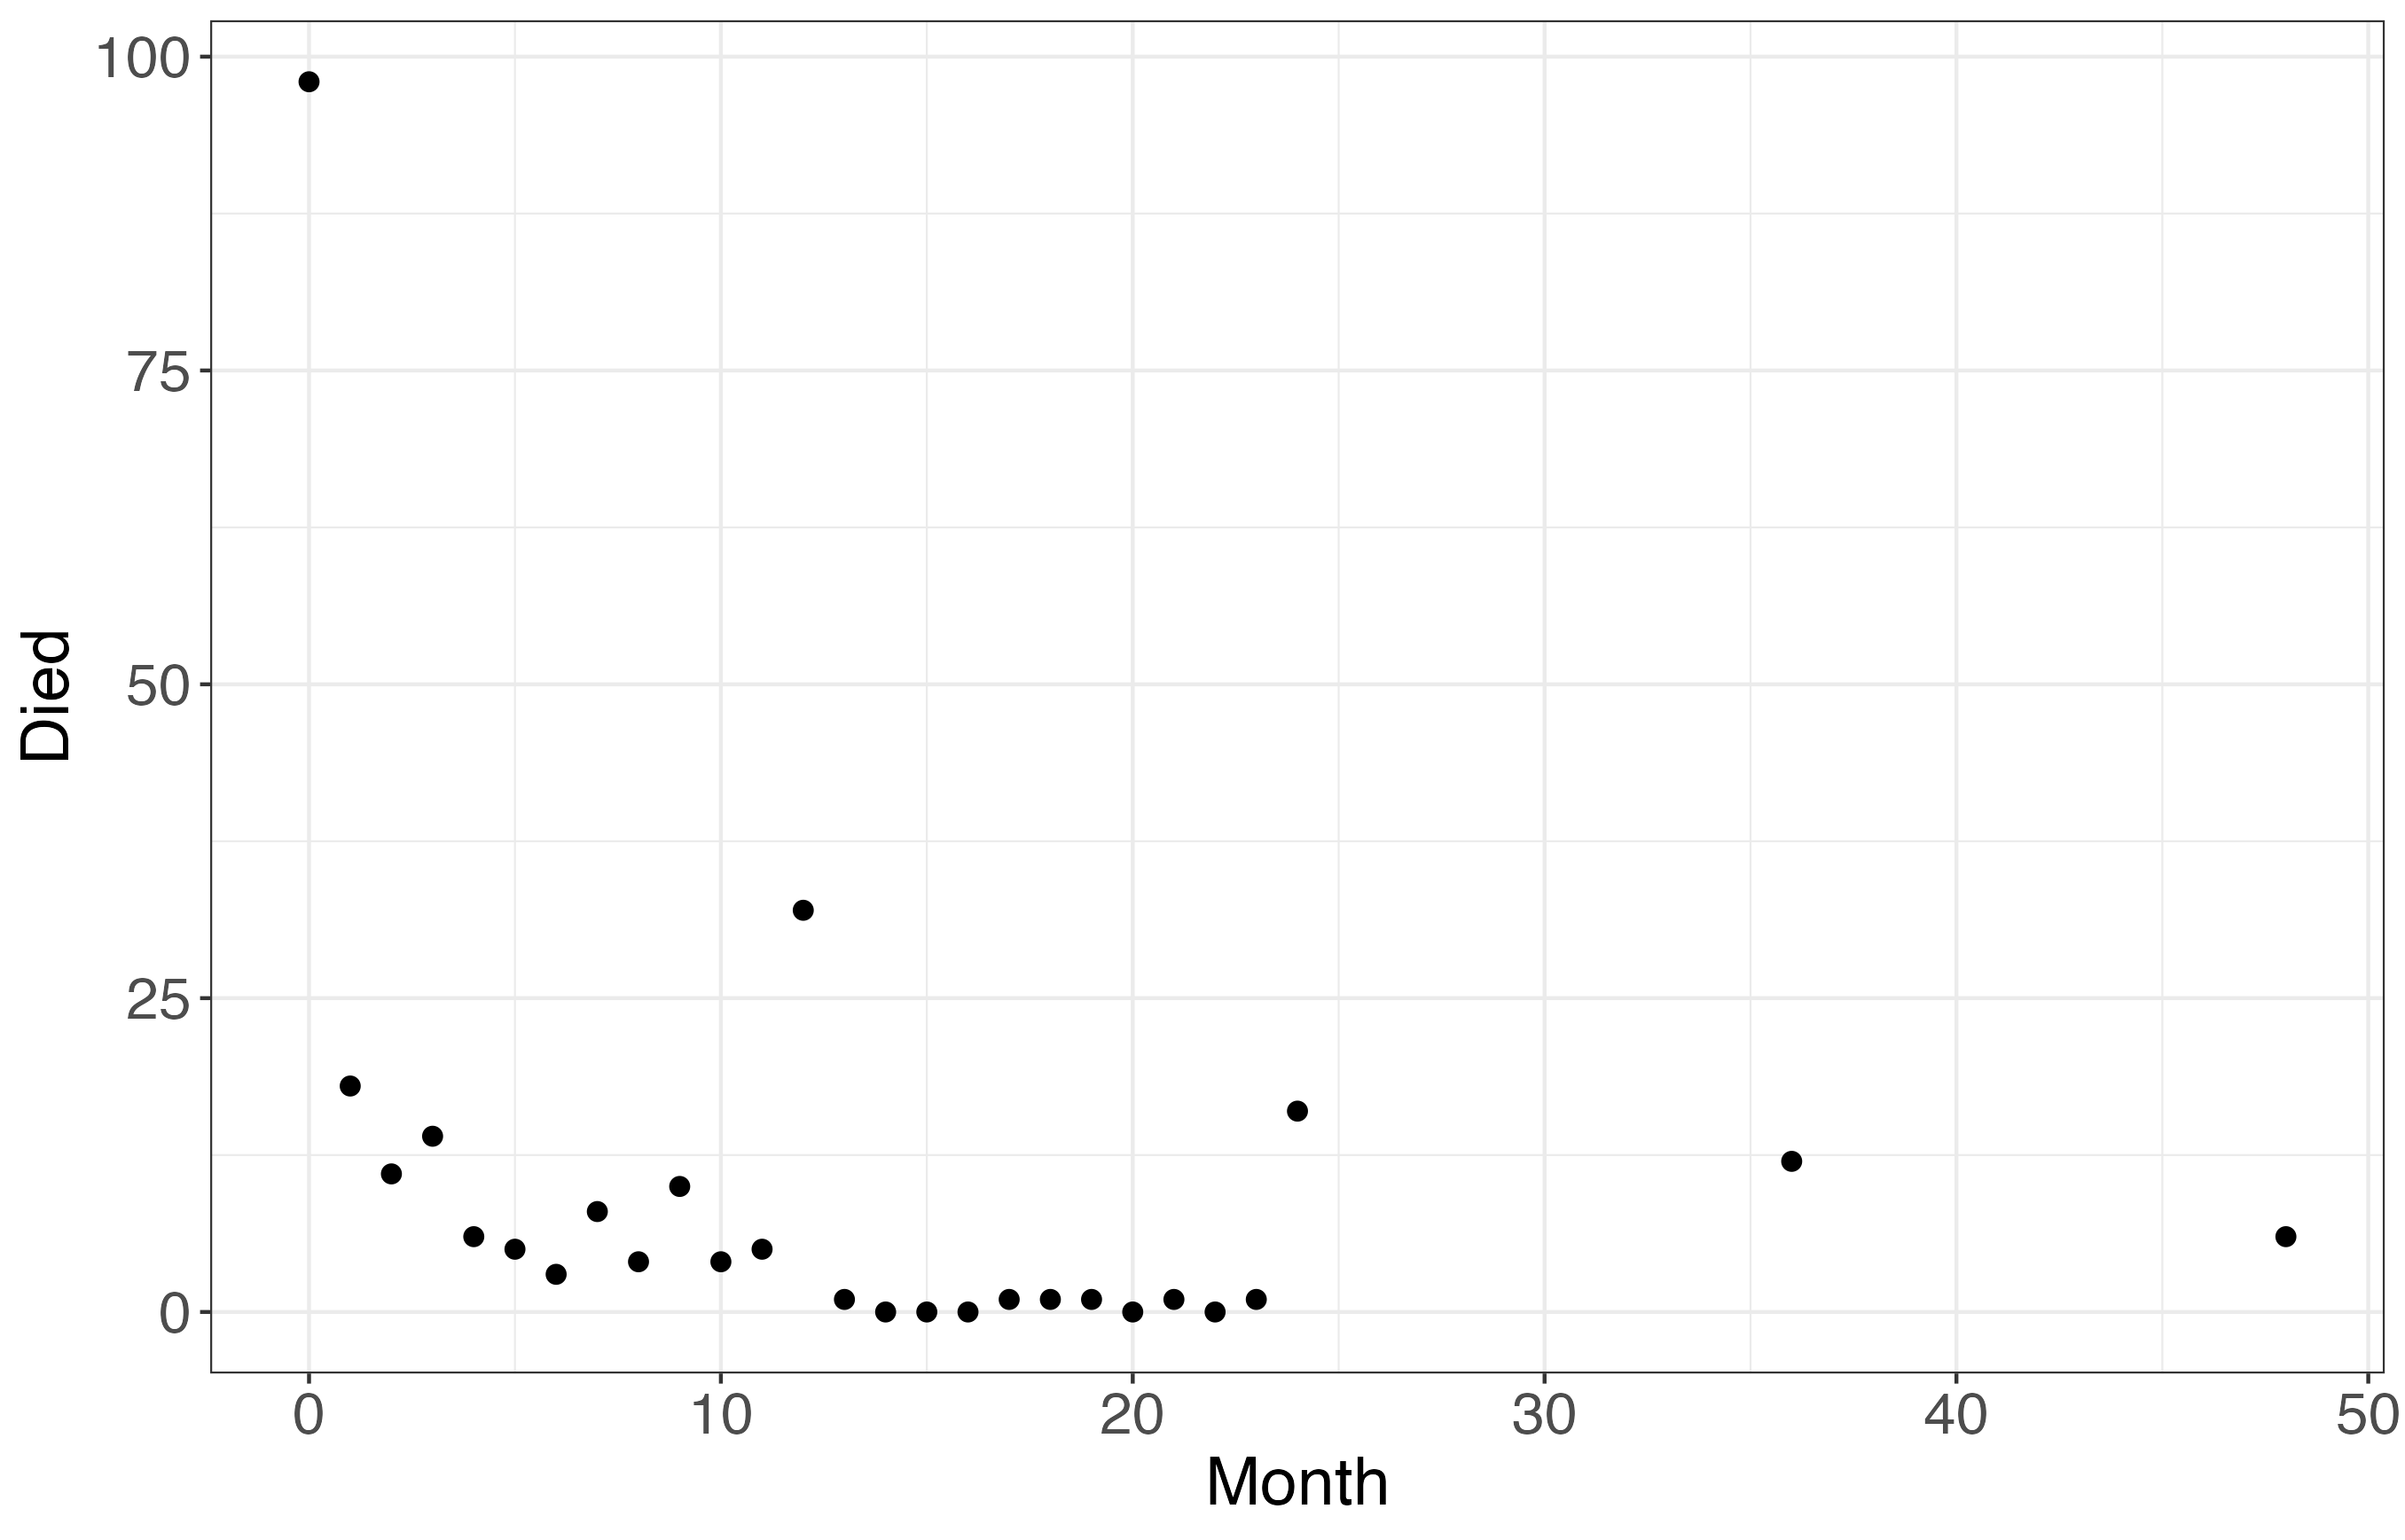
\includegraphics[scale=0.25]{u5mr.png}
\end{frame}

\begin{frame}{Types of Variables: Activity}

\vspace{-5 mm}

\begin{figure}
	\centering 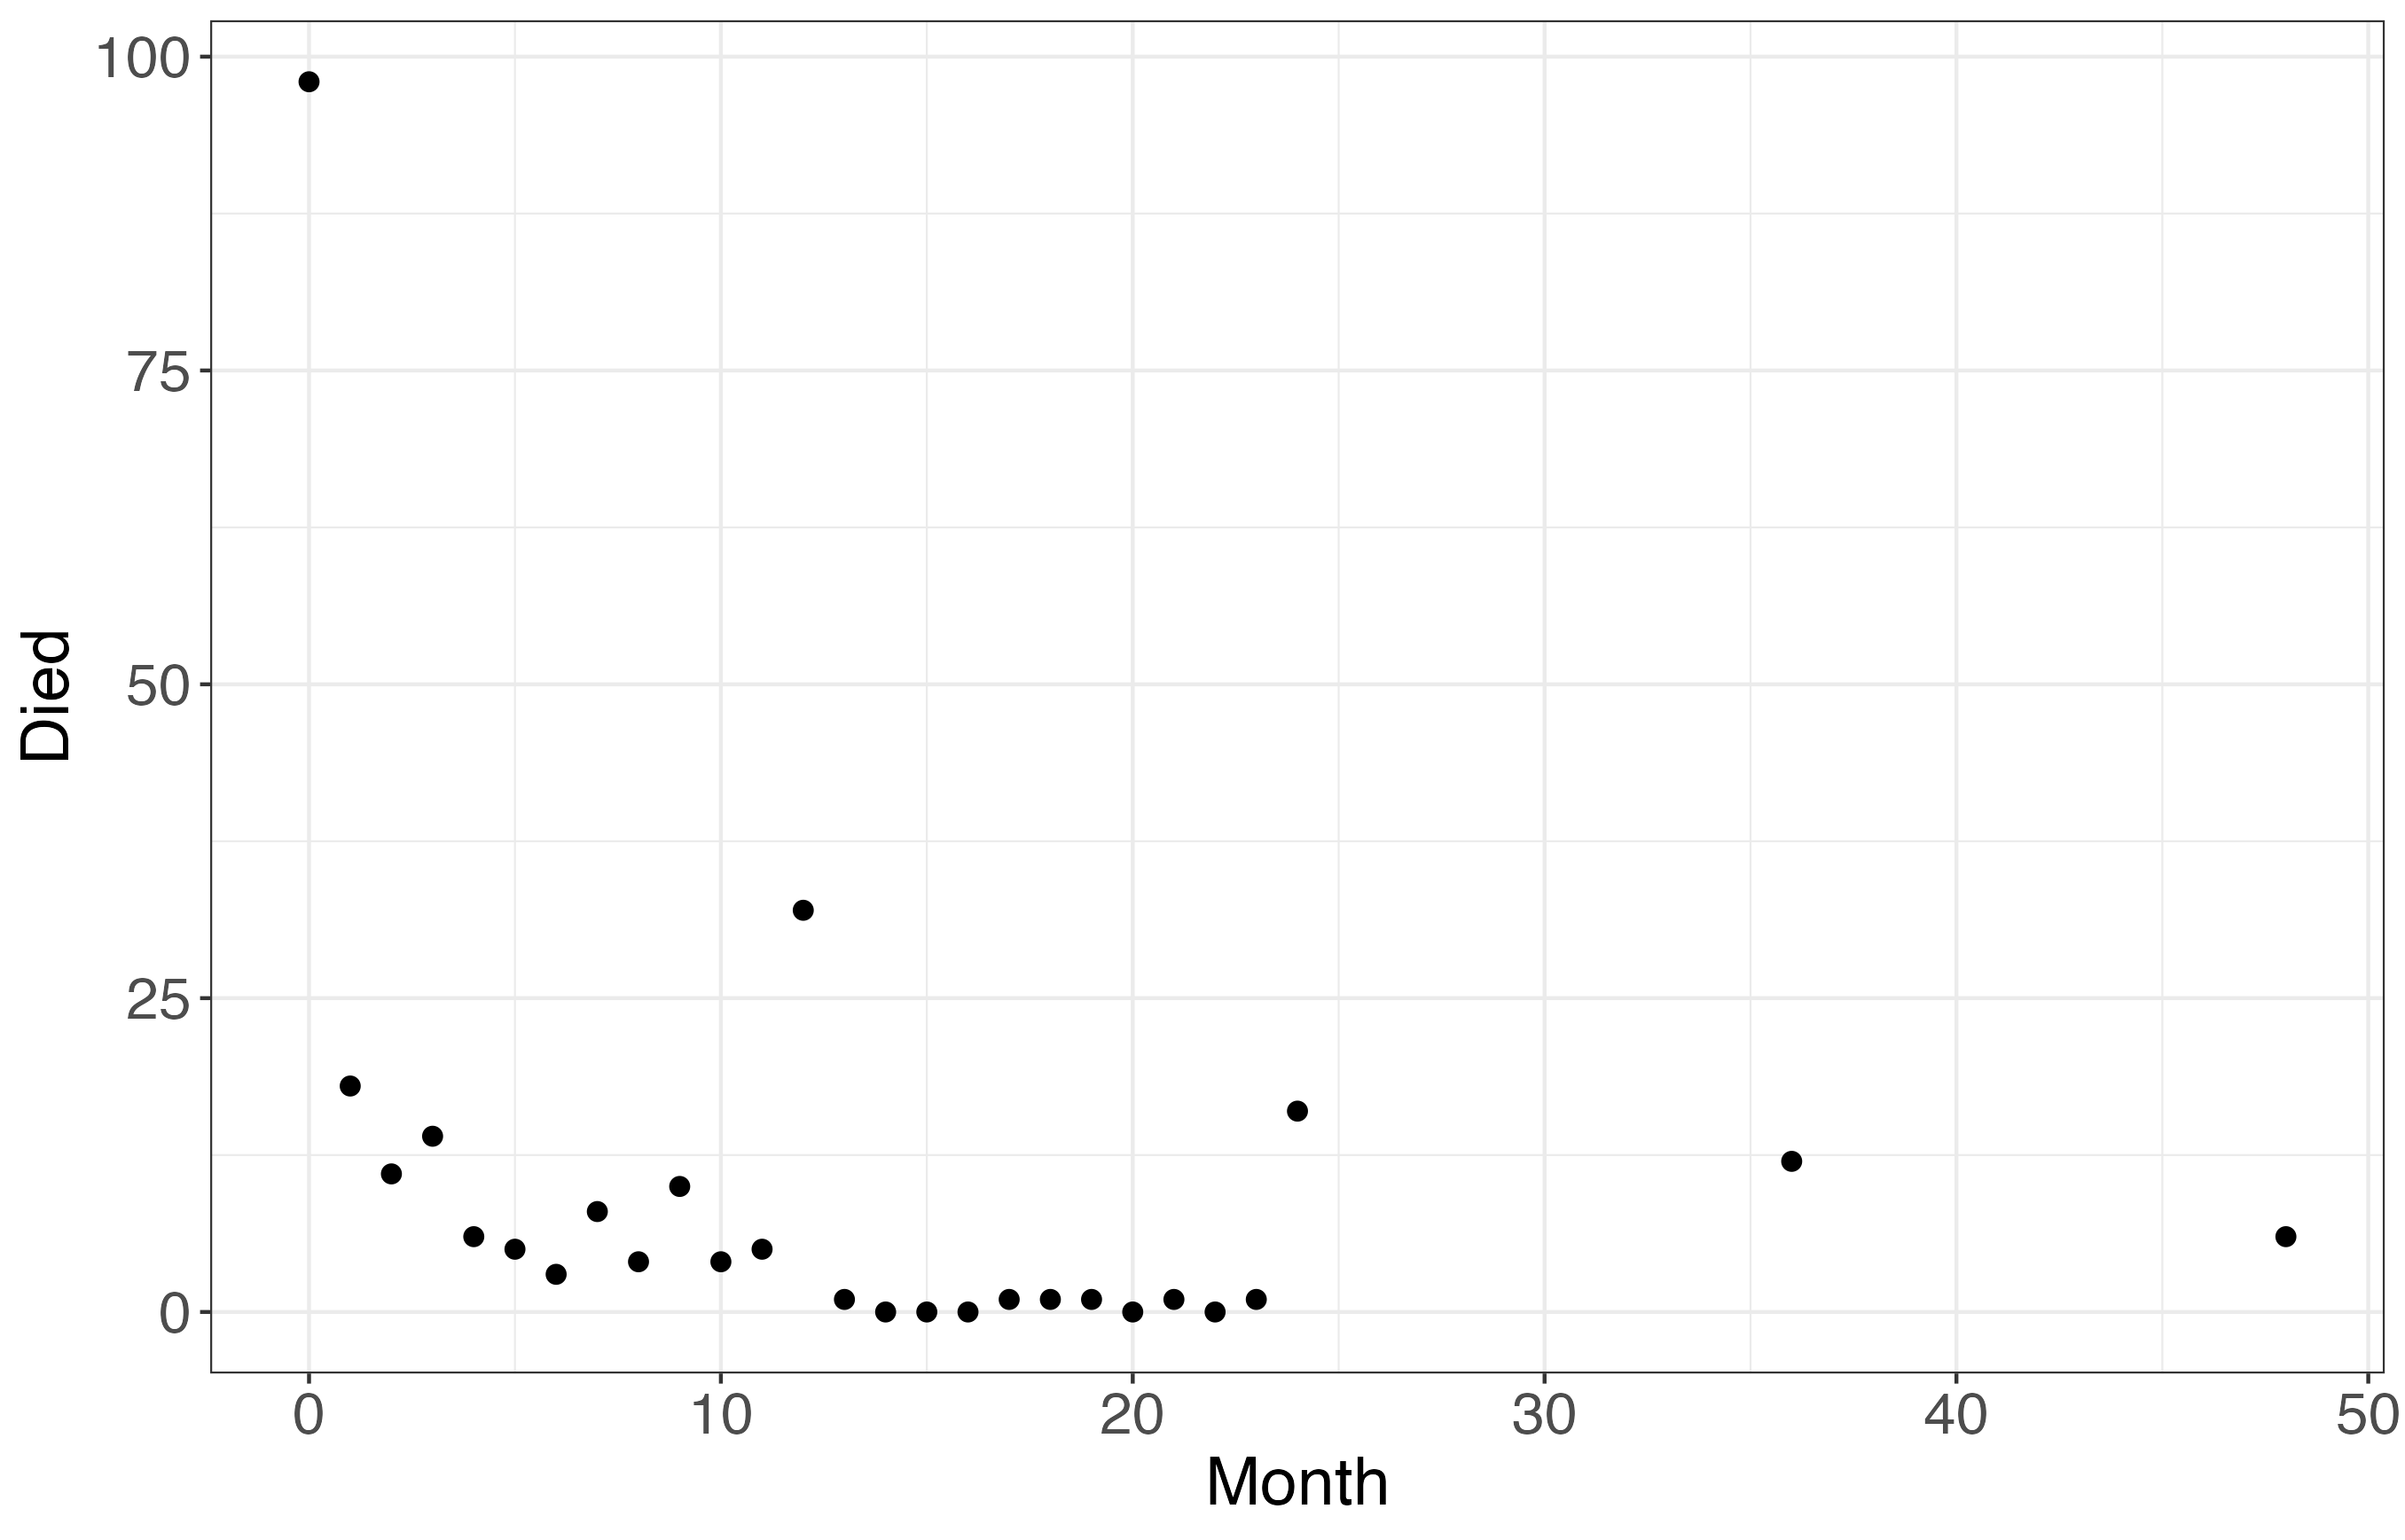
\includegraphics[scale=0.25]{u5mr.png}
\end{figure}
	
\vspace{0.1cm}

\begin{itemize}
	\item Argue why we should consider age at death to be a continuous variable.
	\item Argue why we should consider age at death to be a discrete variable.
	\item Do you notice anything strange about the plot? Does this affect whether or not we should consider age at death to be continuous or discrete?
\end{itemize}

\end{frame}

%\begin{frame}{Types of Variables: Activity}
%
%Argue why we should consider age at death to be a continuous variable.
%	
%	\vspace{0.3cm}
%	
%	\begin{itemize}
%		\item[] \textcolor{blue}{Age is inherently continuous. We could, in theory, have ages recorded with an infinite number of decimal points.}
%	\end{itemize}
%	
%		
%	
%	\vspace{0.3cm}
%	
%	Argue why we should consider age at death to be a discrete variable.
%	
%	\vspace{0.3cm}
%	
%	\begin{itemize}
%		\item[] 	\textcolor{blue}{Age is collected discretely in the survey. According to the survey, children could not be 2.5 years old, for example. }
%	\end{itemize}
%
%	
%
%\end{frame}
%
%\begin{frame}{Types of Variables: Activity}
%
%\vspace{-8 mm}
%
%\begin{figure}
%	\centering 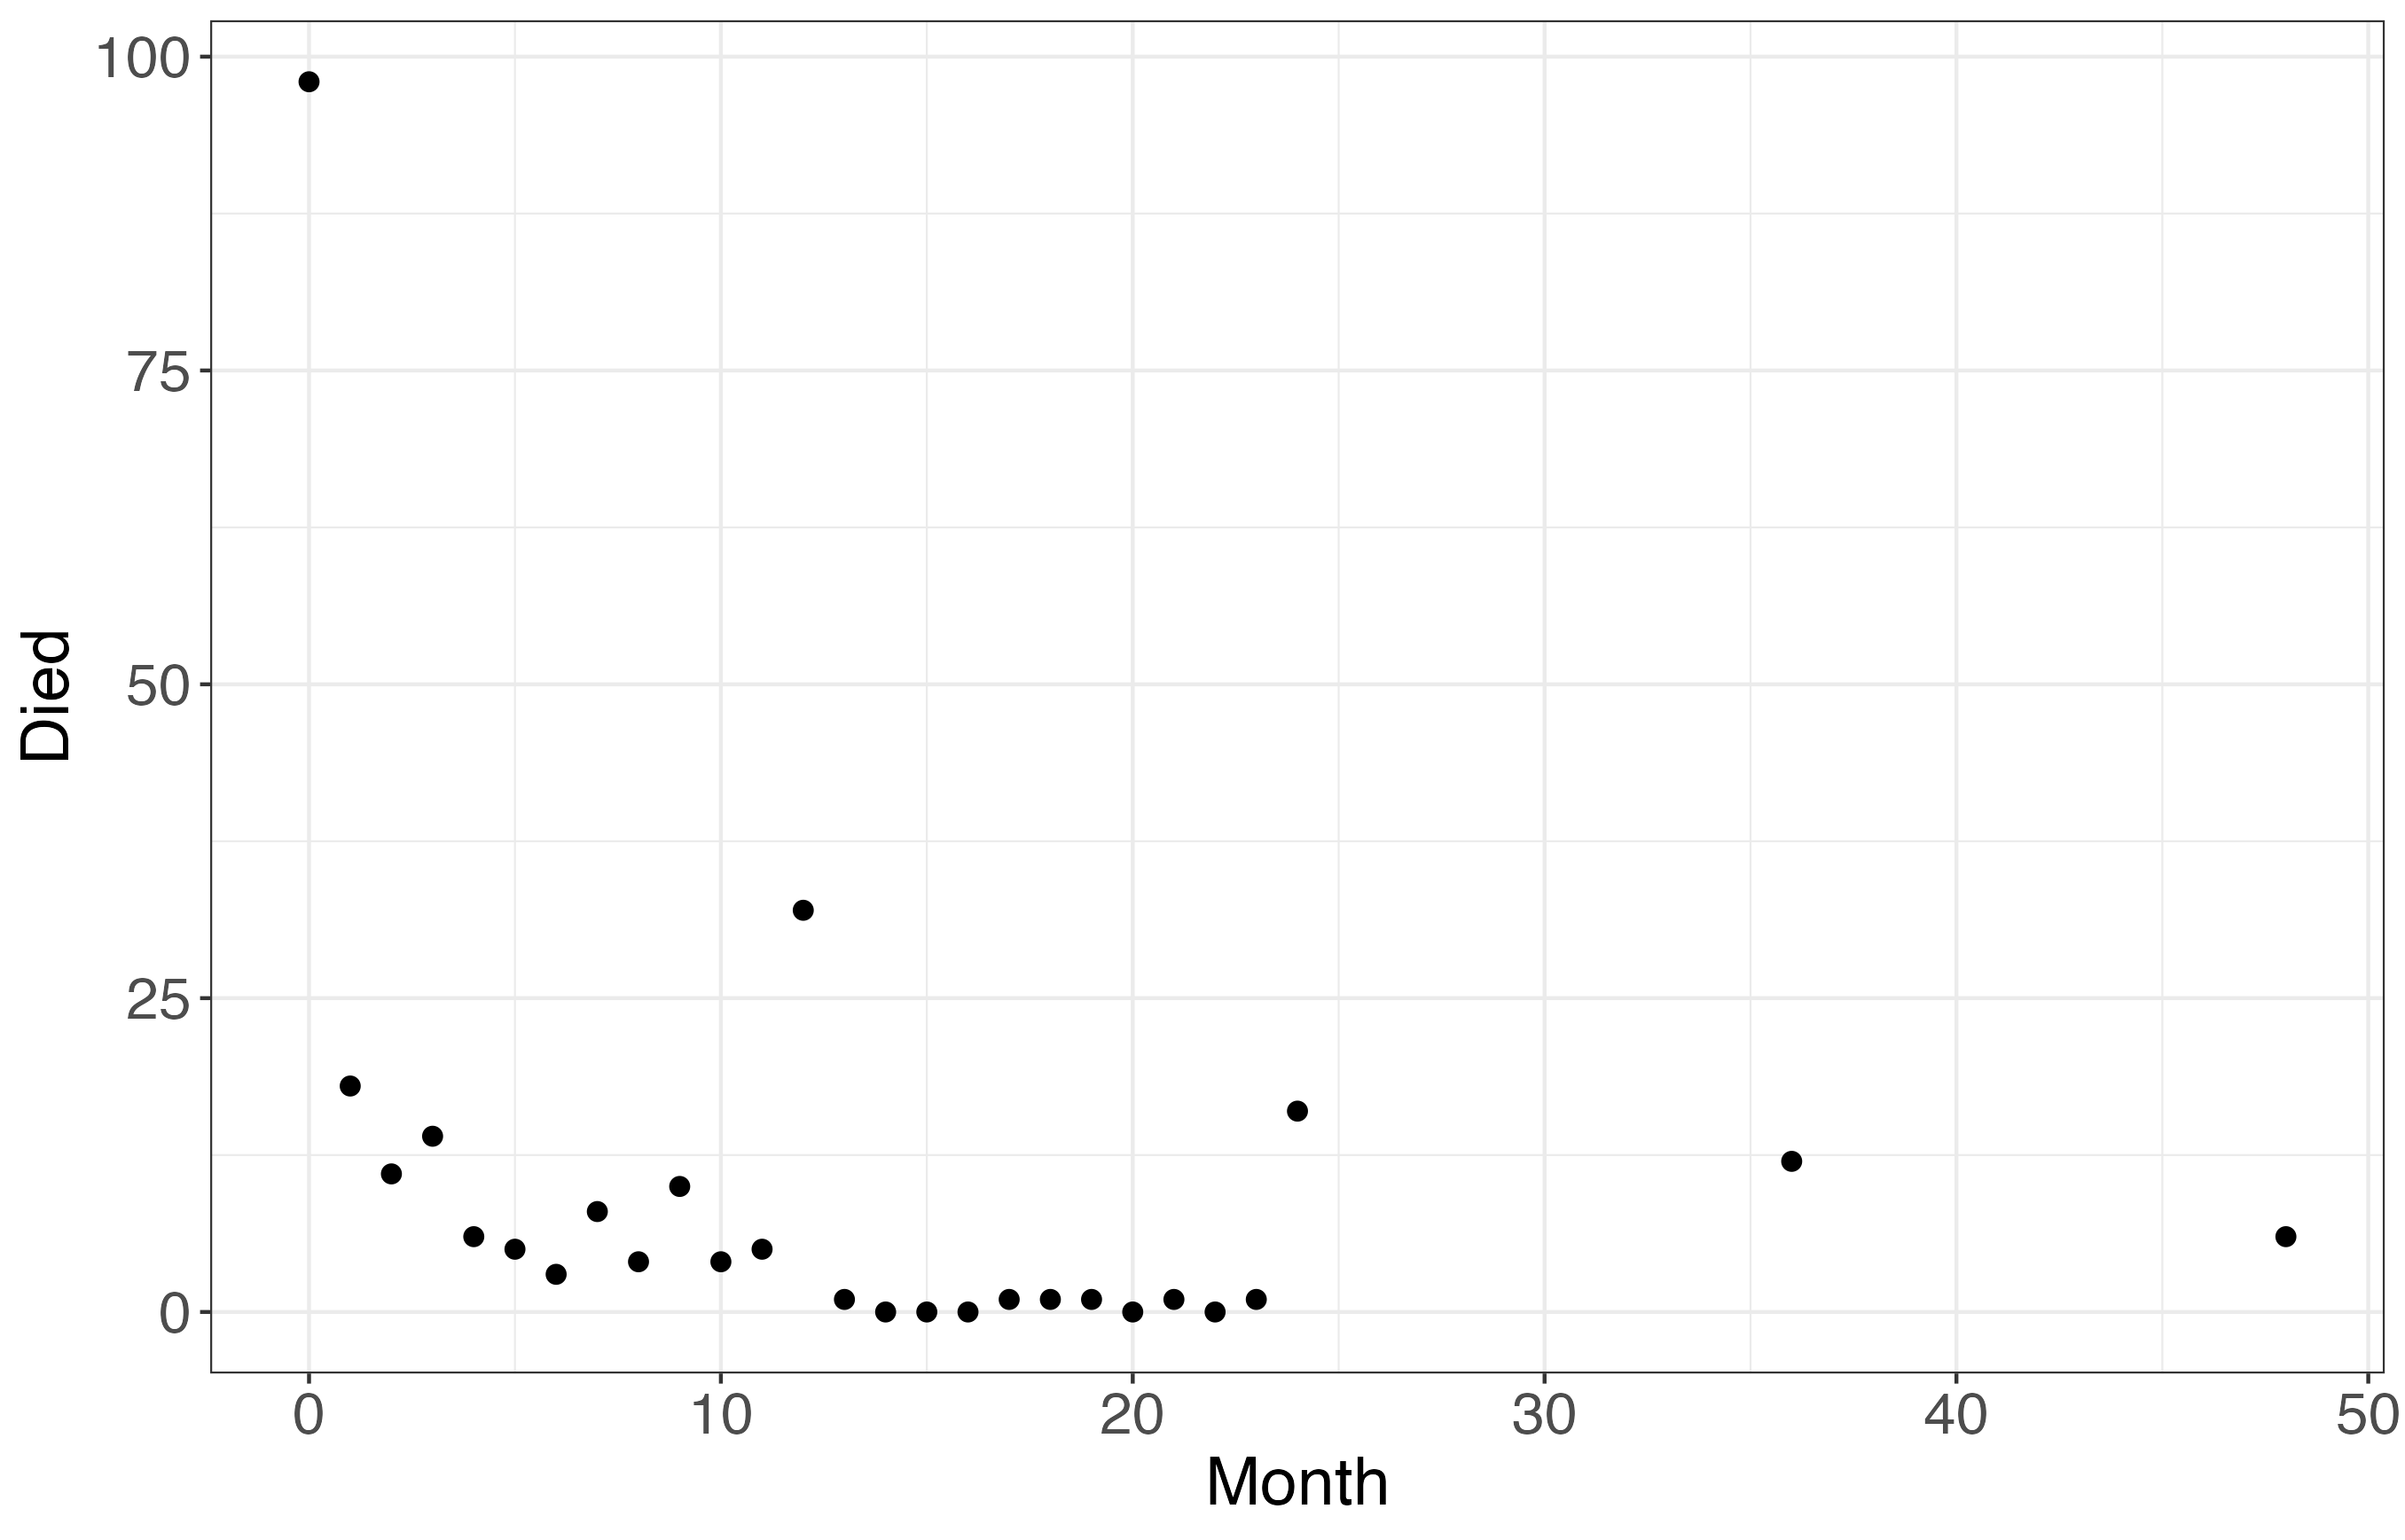
\includegraphics[scale=0.15]{u5mr.png}
%\end{figure}
%	
%{\small Do you notice anything strange about the plot? }
%	
%\smallskip
%	
%\begin{itemize}
%	\item \small \textcolor{blue} {Death counts seem to be higher at exact years than for the months}
%	\smallskip
%		
%	\item \small \textcolor{blue} {For 24 months, 3 years, and 4 years, this is likely due to grouping. If a child died between ages 2.5 - 3.5, they would be recorded as having died at 3 years, so this count is inherently higher since it spans a longer time period than 1 month.} 
%	\smallskip
%	
%    \item \small \textcolor{blue} {However, what about 12 months?}
%	\smallskip
%
%	\item \small \textcolor{blue}{This phenomenon is known as ``age-heaping", and often occurs in surveys where parents do not know the exact age their child was when they died, or when surveyers record dates inexactly. This is essentially a rounding error, where many deaths are recorded at 1 year even though they may have occurred at any time between 0 and 2 years. }
%\end{itemize}	
%	
%\end{frame}
%
%\begin{frame}{Types of Variables: Activity}
%
%
%Considering age to be continuous \textbf{or} discrete in this example are both justifiable conclusions! In general, we'll consider age to be continuous in this class, but in specific scenarios it may make more sense to consider age in discrete groups. 
%\bigskip
%
%In regression models, whether to treat variables are continuous or discrete will be a modeling decision, and may depend on whether the variable is our outcome, the exposure of interest, or another covariate.
%
%\end{frame}

\subsection{Descriptive Statistics}

\begin{frame}{Descriptive statistics vs. Inferential statistics}

	Some terms you should know:
	
	\vspace{0.3cm}
	
	\begin{itemize}
		\item \textcolor{blue}{Descriptive} statistics: summarize or \textcolor{blue}{describe} what's happening \textcolor{blue}{\textbf{in our sample}}
		\item \textcolor{orange}{Inferential} statistics: use our data to \textcolor{orange}{infer} something about \textcolor{orange}{\textbf{our population of interest}}
	\end{itemize}
	
	\vspace{0.3cm}
	
	Often when people talk about ``doing statistics," they're talking about inferential statistics.
	
	\vspace{0.3cm}
	
	But statistics is much more than that. In fact, \textbf{the most important part of statistics} (and often the hardest) \textbf{is translating your scientific question into a statistics question.} Once you've done this, the rest follows.
	
\end{frame}

\begin{frame}{Descriptive Statistics}
Why do we need descriptive statistics?

\vspace{0.3cm}

\begin{itemize}
	\item Making sense of large amounts of data
	\medskip
	\item Checking data quality
	\medskip
	\begin{itemize}
		\item Values outside reasonable range (e.g., height = 9')
		\item Implausible combinations of variables (e.g., positive test for cervical cancer for a person without a cervix)
	\end{itemize}
\medskip

	\item Observe distribution of variables in dataset
	\medskip
	\begin{itemize}
		\item Measures of center and spread
	\end{itemize}
\medskip

	\item Start to understand direction and strength of association
	\medskip
	\begin{itemize}
		\item Descriptive statistics and inferential statistics should contribute to the same story
	\end{itemize}
\end{itemize}

\end{frame}

\begin{frame}{Descriptive Statistics}
Appropriate descriptive statistics will vary depending on what how many variables you want to describe at once, and whether or not you want numerical or graphical summaries.

\vspace{0.3cm}

Outline:
\medskip

\begin{itemize}
	\item Univariate
	\smallskip
	\begin{itemize}
		\item Numerical (categorical variables)
		\smallskip
		\item Numerical (quantitative variables)
	\end{itemize}
\medskip

	\item Stratified/Bivariate
	\begin{itemize}
		\item Numerical summaries, broken down by group
		\smallskip
		\item Graphical
	\end{itemize}
\end{itemize}
\end{frame}

\subsubsection{Univariate}

\begin{frame}{Univariate Descriptive Statistics: Categorical}
\textcolor{blue}{Example:} In our births dataset, we have an indicator variable for whether or not an individual particpated in the First Steps program or not.

\vspace{0.3cm}

Suppose we are interested in knowing how many individuals fall into each group. How would we summarize this data?

\end{frame}

\begin{frame}{Univariate Descriptive Statistics: Categorical}

We could begin by counting up the number of individuals that fall in each category:

\vspace{0.3cm}

\begin{table}
	\centering
	\begin{tabular}{l|r}
		\textbf{First Steps participation} & \textbf{Number of Individuals} \\
		\hline
		Yes & 403\\
		\hline
		No & 2097
	\end{tabular}
\end{table}


\vspace{0.3cm}

*Note that no one in our dataset had a missing value for First Steps participation. If we did have any missing values, we could include this information as an additional ``NA" row in our table

\end{frame}

\begin{frame}{Univariate Descriptive Statistics: Categorical}
We can also report the proportion of individuals that fall in each group:

\vspace{0.3cm}

\begin{table}
	\centering
	\begin{tabular}{l|r}
		\textbf{First Steps participation} & \textbf{Proportion of Individuals (No.)} \\
		\hline
		Yes & 16.1\% (403)\\
		\hline
		No & 83.9\% (2097)
	\end{tabular}
\end{table}

\end{frame}

\begin{frame}{Univariate Descriptive Statistics: Categorical}
Summary should include:

\vspace{0.3cm}

\begin{itemize}
	\item Number and percent in each group
	\medskip
	\item If binary, only need to summarize one group
	\smallskip
	\begin{itemize}
		\item The other can be inferred (for example, we had 16.1\% of individuals participate in First Steps, so 100 - 16.1 = 83.9\% did not.)
	\end{itemize}
\medskip
	\item Also good to summarize missing data
	\smallskip
	\begin{itemize}
		\item e.g., \# and proportion of missing values
	\end{itemize}
\end{itemize}
\medskip


\begin{table}
	\centering
	\begin{tabular}{l|r}
		\textbf{First Steps participation} & \textbf{Proportion of Individuals (No.)} \\
		\hline
		Yes & 16.1\% (403)\\
	\end{tabular}
\end{table}
	
\end{frame}

\begin{frame}{Univariate Descriptive Statistics: Quantitative}

\textcolor{blue}{Example:} The primary outcome of interest in our births dataset is birthweight, recorded in grams. The data for birthweight looks like:

\vspace{0.3cm}

\begin{table}
	\centering
	\begin{tabular}{l|r}
		\textbf{Individual ID} & \textbf{Birthweight (grams)} \\
		\hline
		1 & 3118\\
		\hline
		2 & 3466\\
		\hline
		3 & 3147 \\
		\hline 
		\vdots & \vdots \\
		\hline
		2498 & 3005 \\
		\hline 
		2499 & 1644 \\
		2500 & 3317
	\end{tabular}
\end{table}

\vspace{0.3cm}

What information may be useful to know?

\end{frame}

\begin{frame}{Univariate Descriptive Statistics: Quantitative}

\vspace{-5 mm}

How many individuals are in our dataset?

\begin{itemize}
	\item[] \textcolor{blue}{2500 individuals in our dataset.} (\texttt{R} code: \texttt{nrow(births)})
\end{itemize}

Do any individuals have missing values for birthweight?

\begin{itemize}
	\item[] \textcolor{blue}{No!} (\texttt{R} code: \texttt{summary(births\$bwt)})
\end{itemize}

Measures of center? (\texttt{R} code: \texttt{summary(births\$bwt)})

\begin{itemize}
	\item[] \textcolor{blue}{Mean birthweight is 3414 grams.}
	\item[] \textcolor{blue}{Median birthweight is 3444 grams.}
\end{itemize}

Measures of spread?

\begin{itemize}
	\item[] \textcolor{blue}{Sample standard deviation is 559 grams.} 
	\begin{itemize}
	\item[] (\texttt{R} code: \texttt{sd(births\$bwt,na.rm = TRUE)})
	\end{itemize}
	\item[] \textcolor{blue}{Interquartile range (IQR) is (3096 grams, 3766 grams) (Q1, Q3)}
	\begin{itemize}
		\item[] (\texttt{R} code: \texttt{summary(births\$bwt)})
	\end{itemize}
	\item[] \textcolor{blue}{Range is (255 grams, 5175 grams) (The smallest baby to ever survive weighed around 212 grams)}
	\begin{itemize}
		\item[] (\texttt{R} code: \texttt{summary(births\$bwt)})
	\end{itemize}
\end{itemize}


\end{frame}
	
\begin{frame}{Univariate Descriptive Statistics: Quantitative}
Summary should include (some of):

\vspace{0.3cm}

\begin{itemize}
	\item Sample size / number of observations
	\medskip
	\item Number of missing observations
	\medskip
	\item Measures of center:
	\begin{itemize}
			\smallskip
		\item Sample mean
			\smallskip
		\item Sample median
	\end{itemize}
\medskip
	\item Measures of spread:
	\begin{itemize}
		\smallskip
		\item Sample standard deviation
			\smallskip
		\item Interquartile range (IQR): (Q1, Q3) or (Q3 - Q1)
			\smallskip
		\item Range: (Min, Max) or (Max - Min)
	\end{itemize}
\end{itemize}

\end{frame}

\begin{frame}{Univariate Descriptive Statistics: Graphical}
For categorical variables, we can make barplots:

\vspace{0.3cm}

\centering 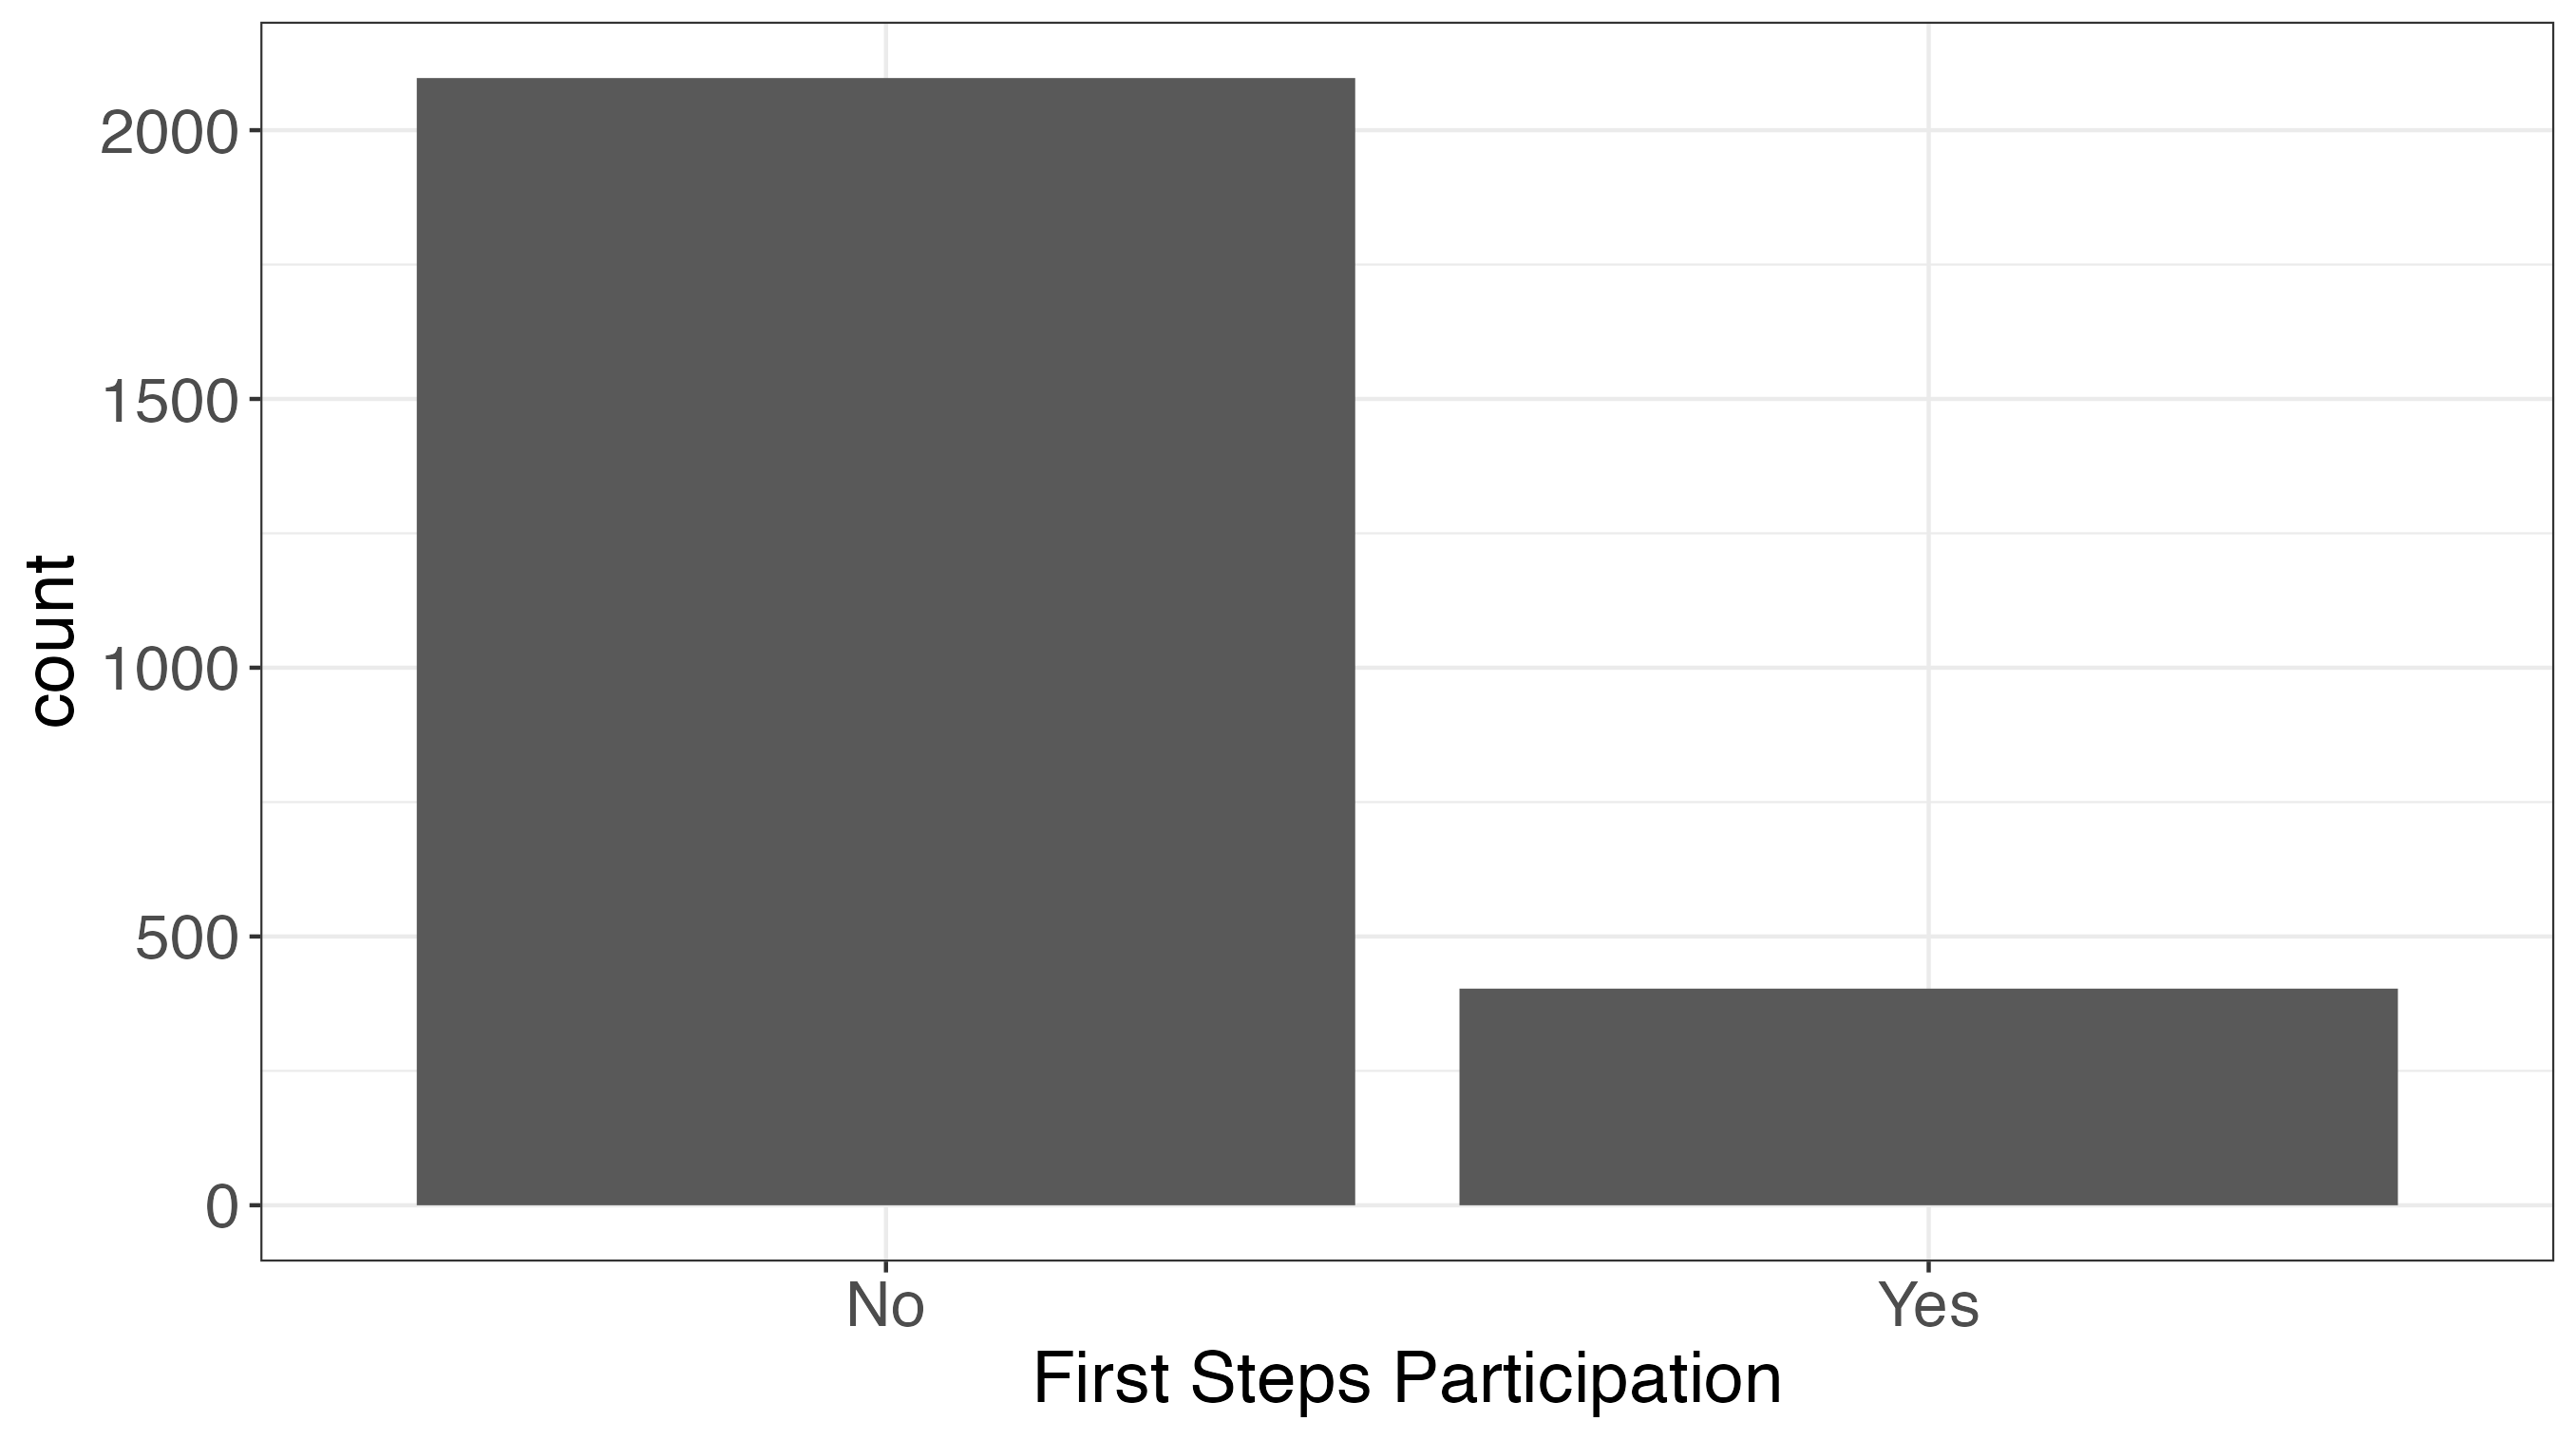
\includegraphics[scale=0.4]{fs_bar.png}

\end{frame}

\begin{frame}{Univariate Descriptive Statistics: Graphical}
For quantitative variables, we can make histograms and boxplots. Histograms are useful for describing the shape of the distribution of a variable, and boxplots are useful for seeing central tendency (and sometimes outliers):

\vspace{0.4cm}

\begin{figure}
	\centering
	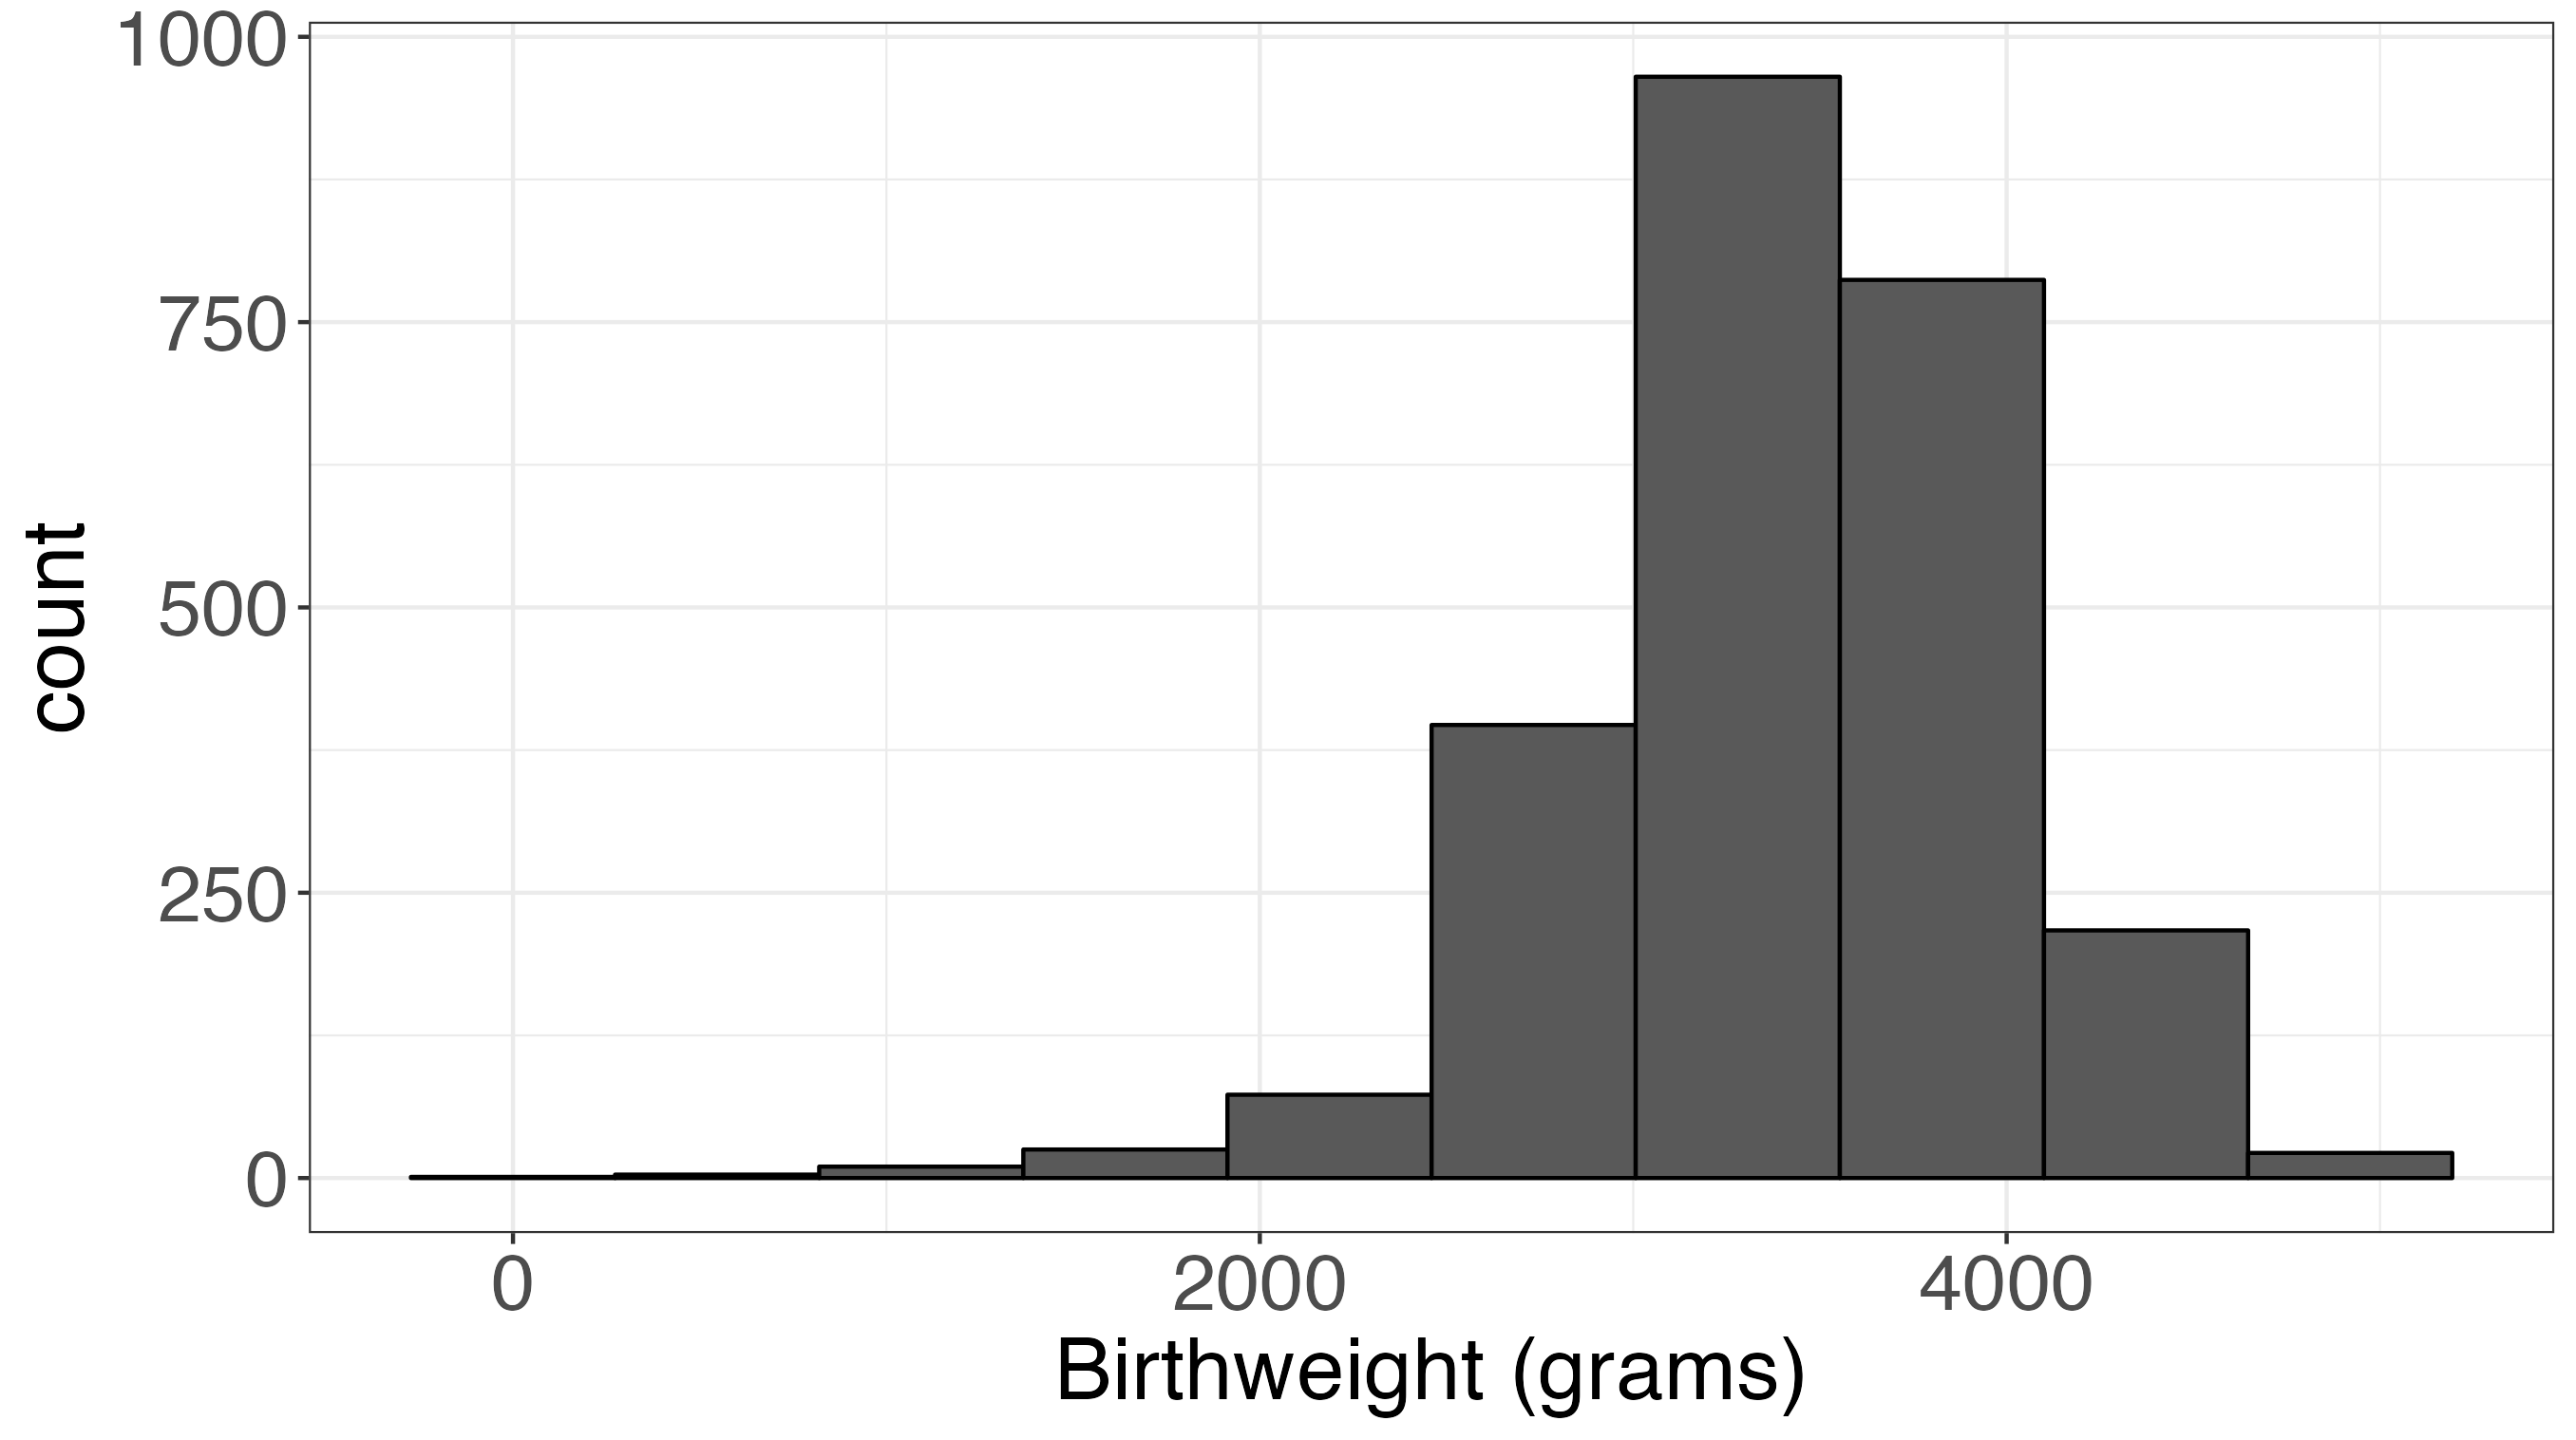
\includegraphics[scale=0.2]{fs_hist.png}
	\hspace{0.2cm}
	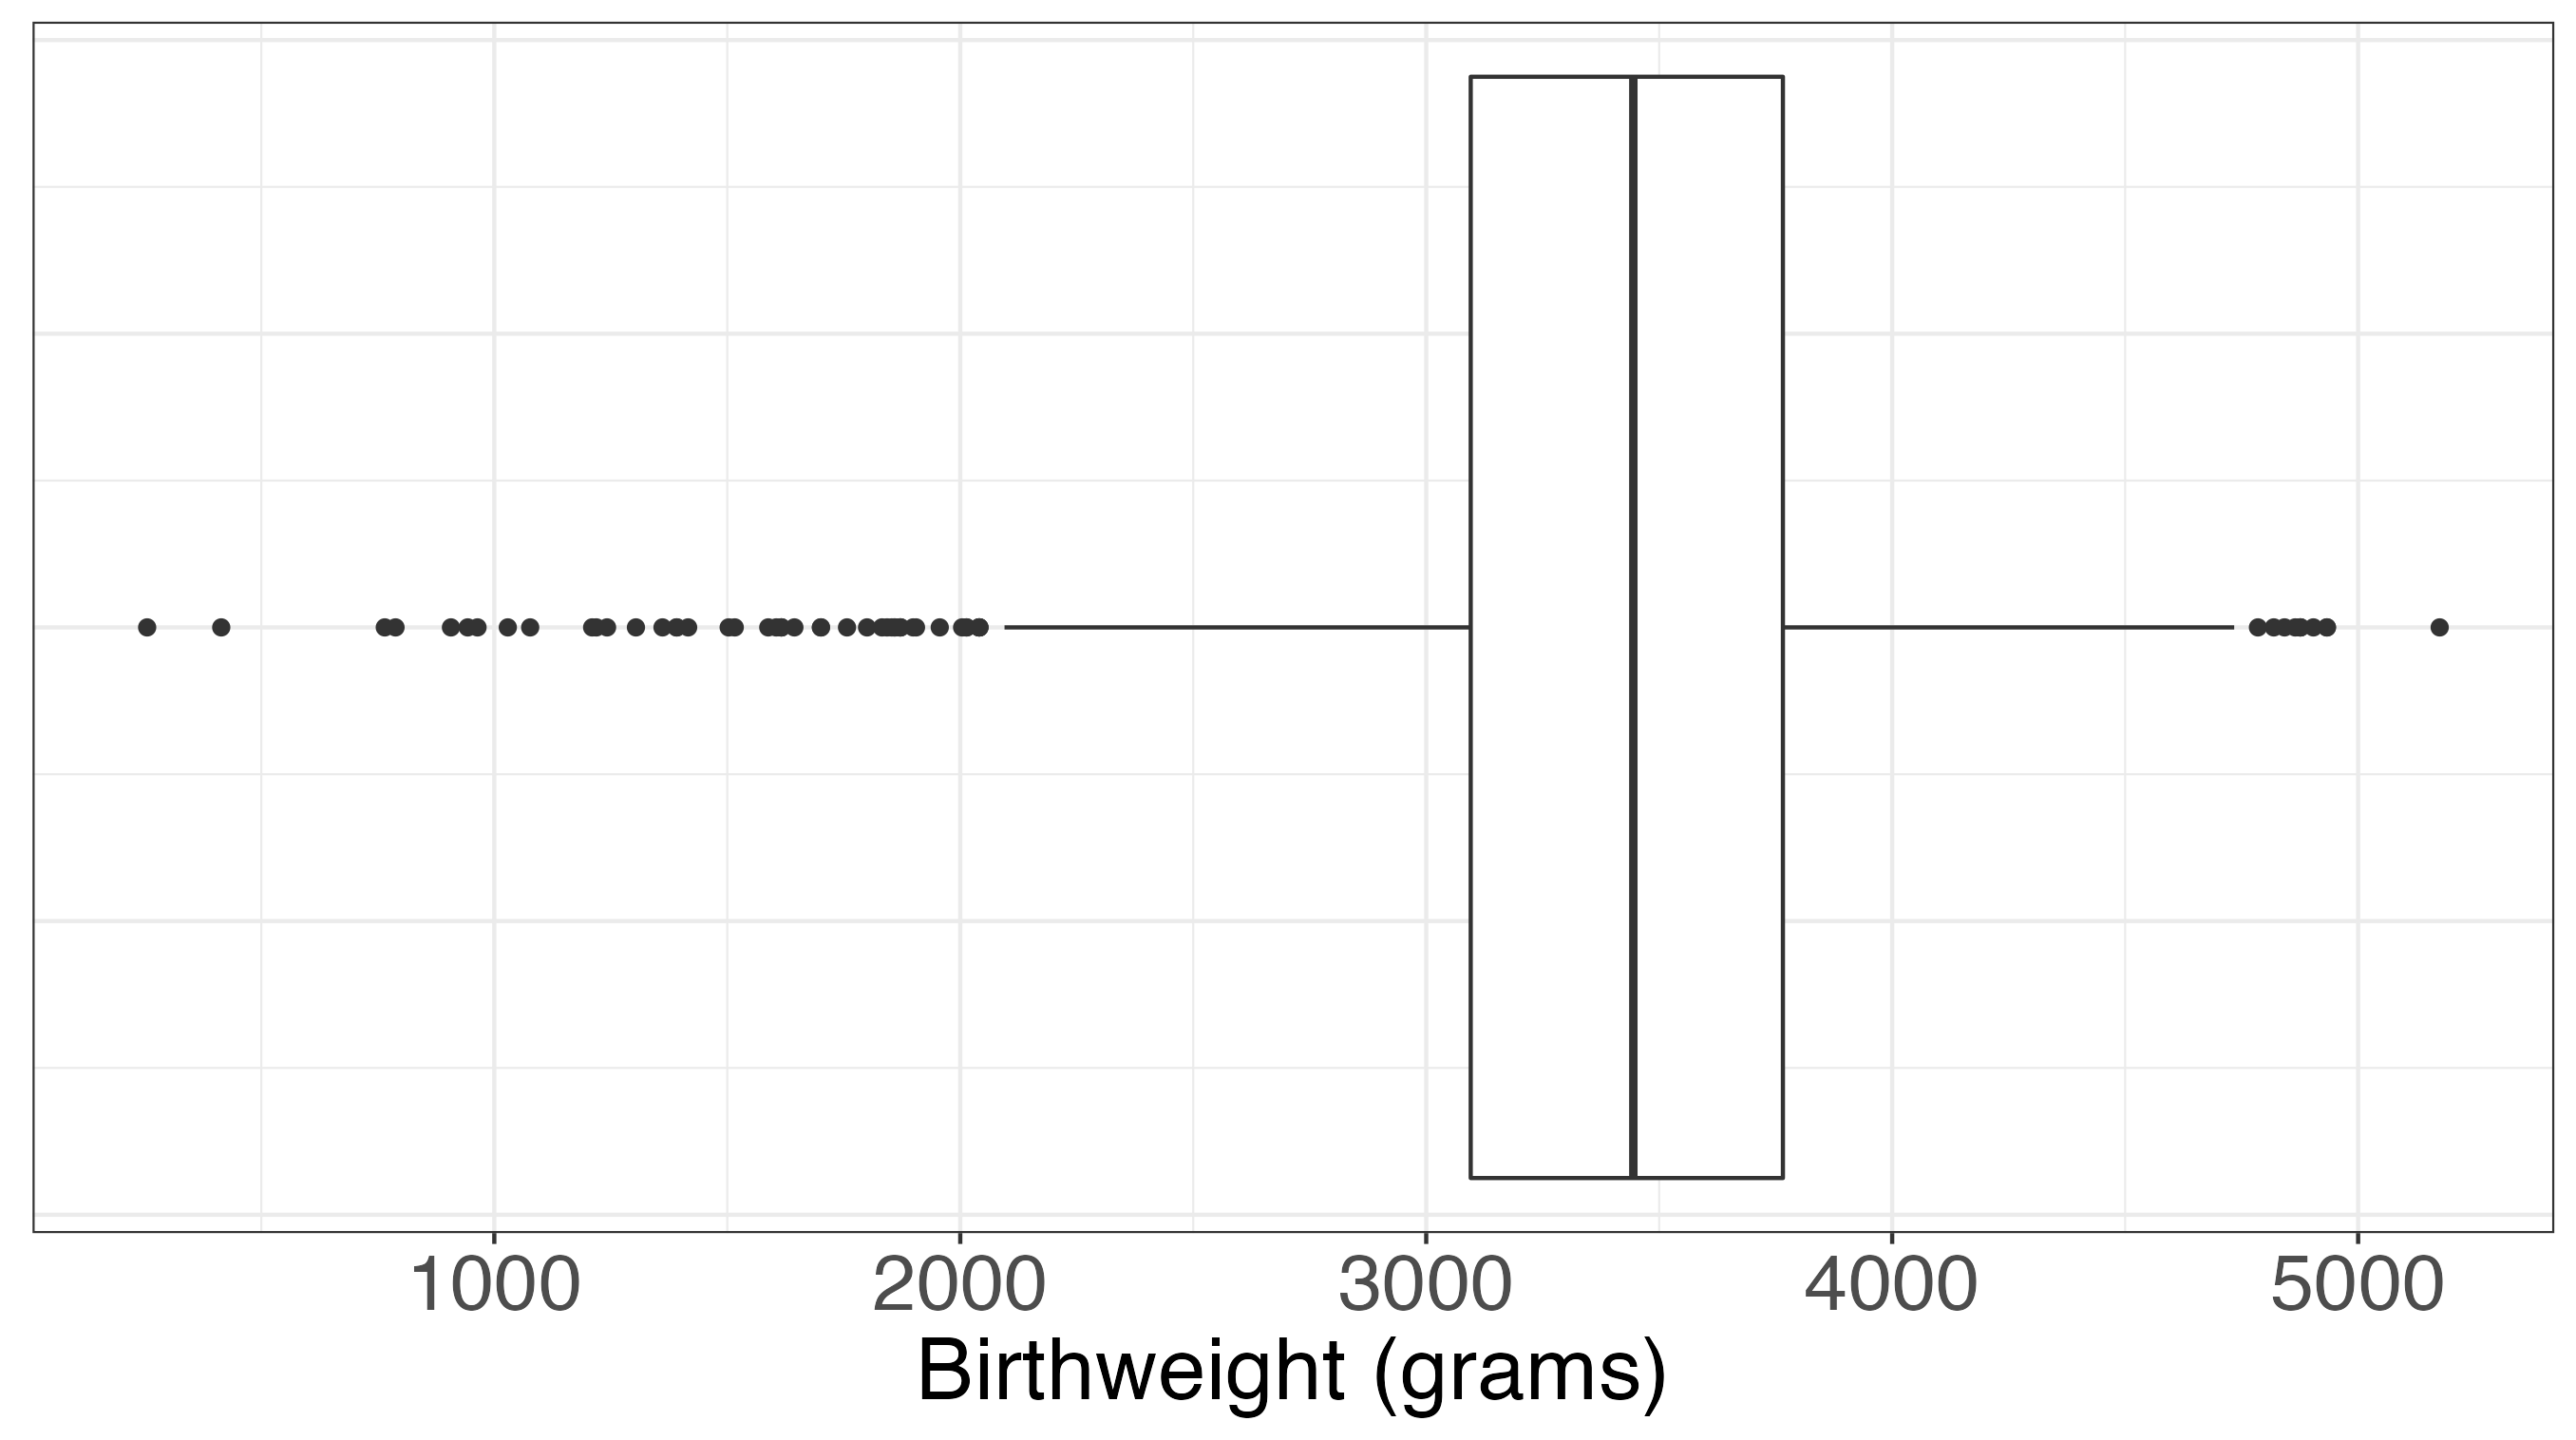
\includegraphics[scale=0.2]{fs_box.png}
\end{figure}

\end{frame}

\subsubsection{Stratified/Bivariate}

\begin{frame}{Stratified Descriptive Statistics: Graphical}
Sometimes we're interested in the distribution of a variable within certain subgroups, rather than across all the data:

\vspace{0.3cm}

\begin{itemize}
	\item e.g., how does the distribution of birthweights differ between individuals who pariticipated in First Steps and those who did not?
\end{itemize}

\vspace{0.3cm}

Stratified descriptive statistics can help us:

\vspace{0.3cm}

\begin{itemize}
	\item Understand the role of the stratification variable
	\medskip
	\item Begin to demonstrate the association between the two variables
\end{itemize}

\end{frame}

\begin{frame}{Stratified Descriptive Statistics: Graphical}

How does the distribution of birthweights differ between individuals who participated in First Steps and those who did not? We can make histograms for each category of individuals:

\vspace{0.3cm}

\centering 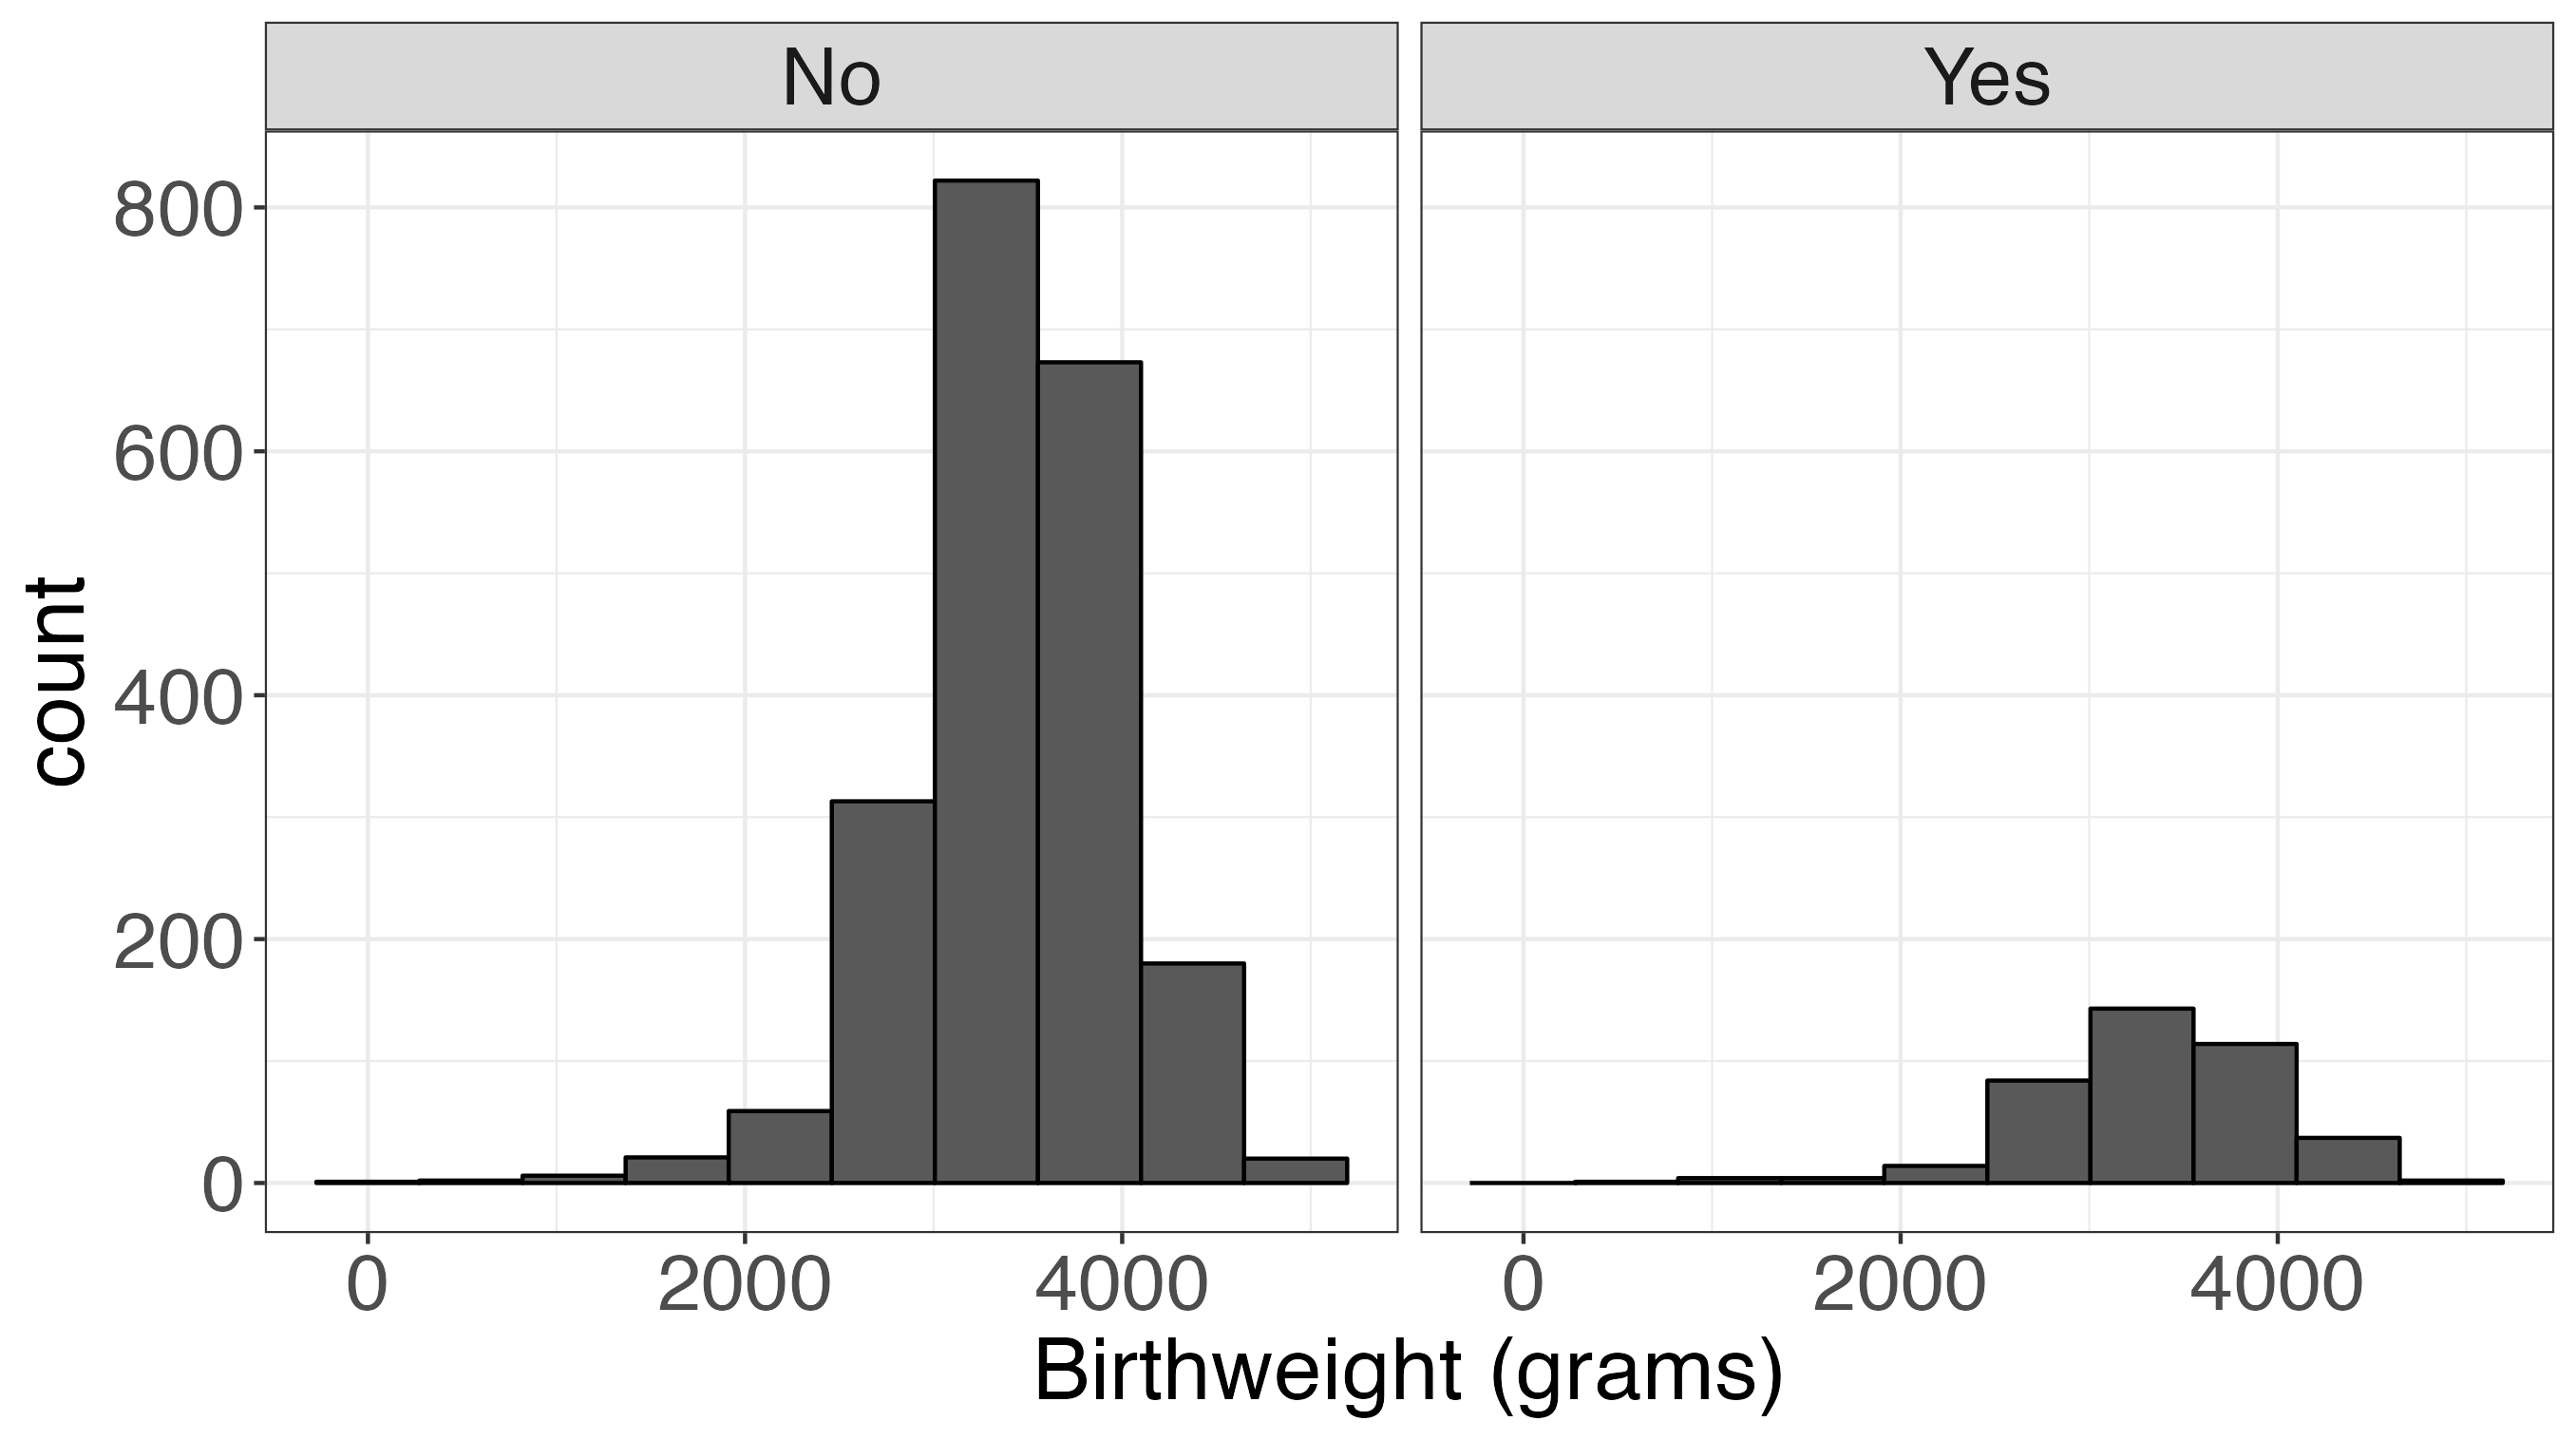
\includegraphics[scale=0.3]{fs_hist_firstep.png}

\end{frame}

\begin{frame}{Stratified Descriptive Statistics: Graphical}
We can also use side-by-side boxplots rather than side-by-side histograms. It may be easier to see the median birthweight is slightly lower in individuals who participated in First Steps:

\vspace{0.3cm}

\centering 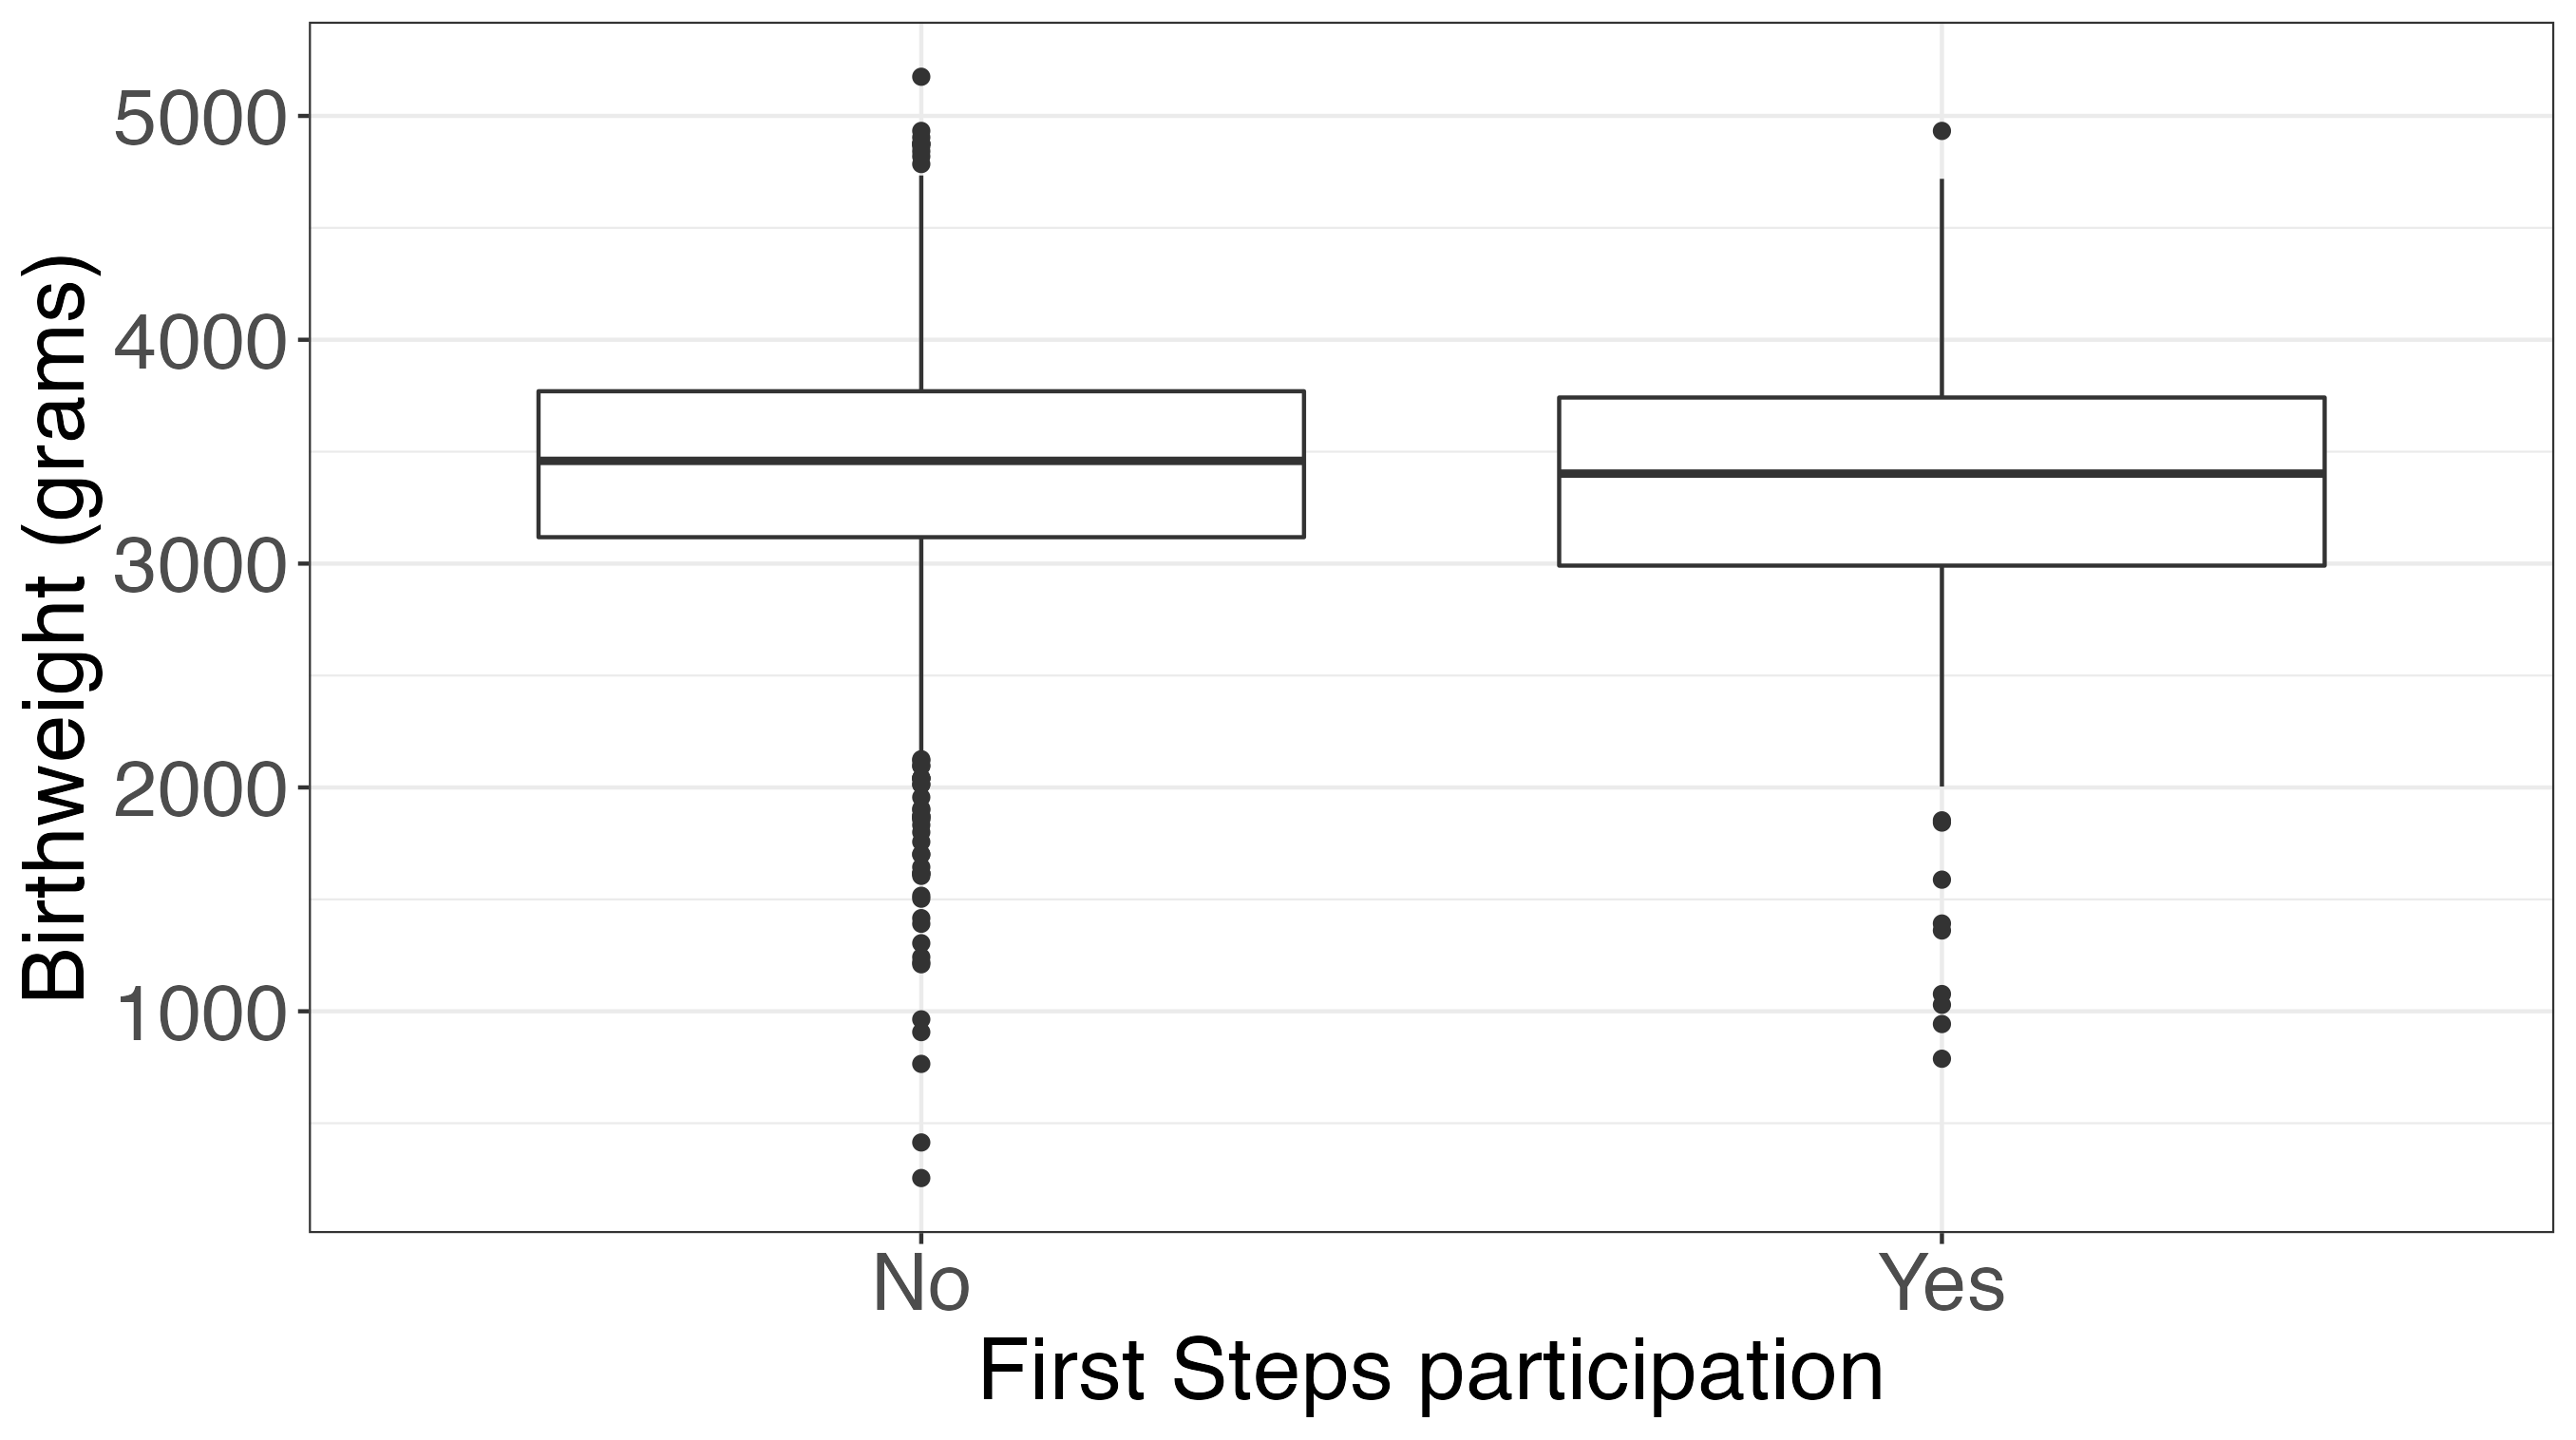
\includegraphics[scale=0.3]{fs_box_firstep.png}
\end{frame}

\begin{frame}{Stratified Descriptive Statistics: Graphical}
Scatterplots are a useful tool for summarizing the relationship between two quantitative variables. Below we plot age in years vs. birthweight in grams for all individuals in our births dataset:

\vspace{0.3cm}

\centering 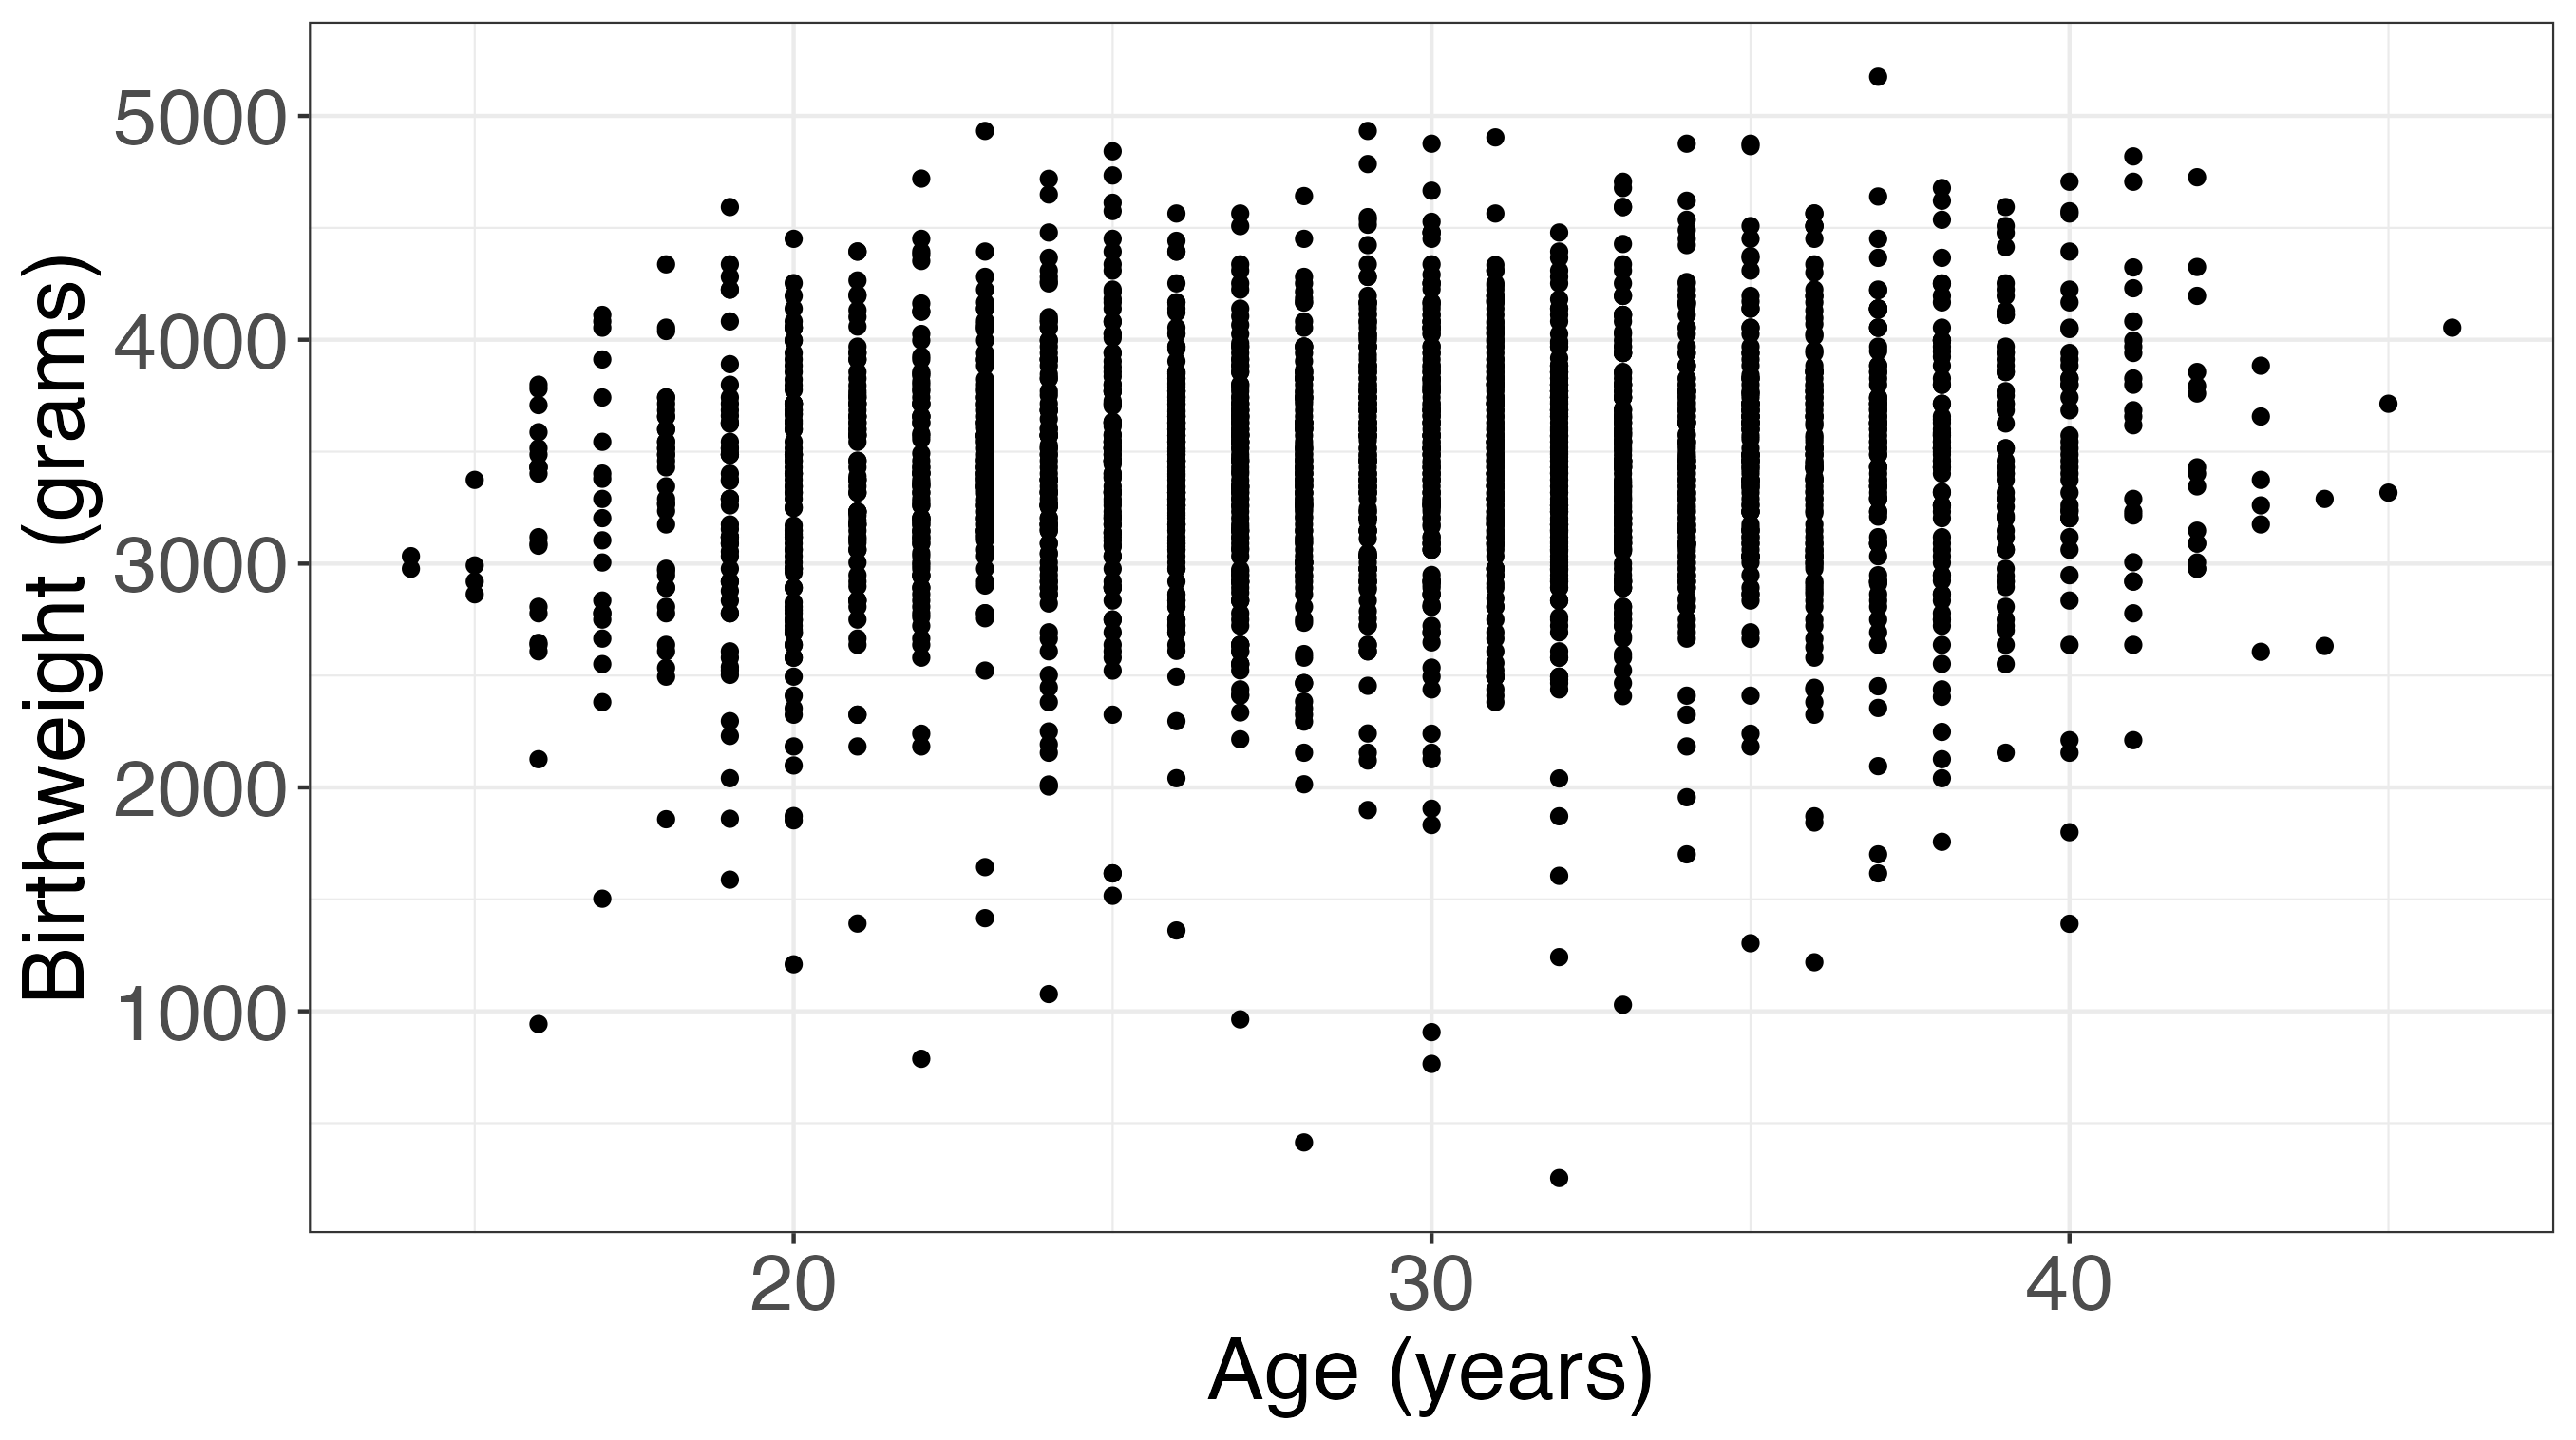
\includegraphics[scale=0.3]{fs_scatter.png}

\end{frame}

\begin{frame}{Descriptive Statistics in R}
This is just a small taste of the many possibilities when it comes to tools for summarizing data.

\vspace{0.3cm}

We’ll spend more time discussing descriptive statistics in Discussion Section, including how to generate numerical summaries and graphical summaries like these (or better ones!) in \texttt{R}.

\vspace{0.3cm}

You’ll also get practice on homework assignments and your data analysis project!

\end{frame}

\begin{frame}[c]
\centering \huge Any Questions?
\end{frame}

\section{Statistical inference}

\begin{frame}{Statistical Inference} 
Why do we do statistics?
\medskip
\begin{itemize}
	\item We can't (usually) measure everyone in our \textbf{population}
	\smallskip
	\begin{itemize}
		\item \textbf{Example}: all pregnant individuals in King County
	\end{itemize}
\smallskip
	\item Instead, we take a \textbf{sample}
	\begin{itemize}
		\smallskip
		\item \textbf{Example}: 2500 pregnant individuals with singleton births
		\smallskip
		\item Note: important to sample well so that the sample truly reflects (is \textbf{representative} of) our population of interest
	\end{itemize}
\smallskip

	\item We hope that what we estimate from the sample also applies to the population
	\smallskip
	
	\begin{itemize}
		\item The process of translating from the \textbf{sample} to the \textbf{population} is \textbf{statistical inference}
		\smallskip
		
		\item What we estimate in the sample = \textbf{estimate} or \textbf{statistic}
		\smallskip
		
		\item Corresponding value in population = \textbf{parameter}
	\end{itemize}
\end{itemize}
\end{frame}

\begin{frame}[c]{Statistical Inference: Work Flow}
\centering 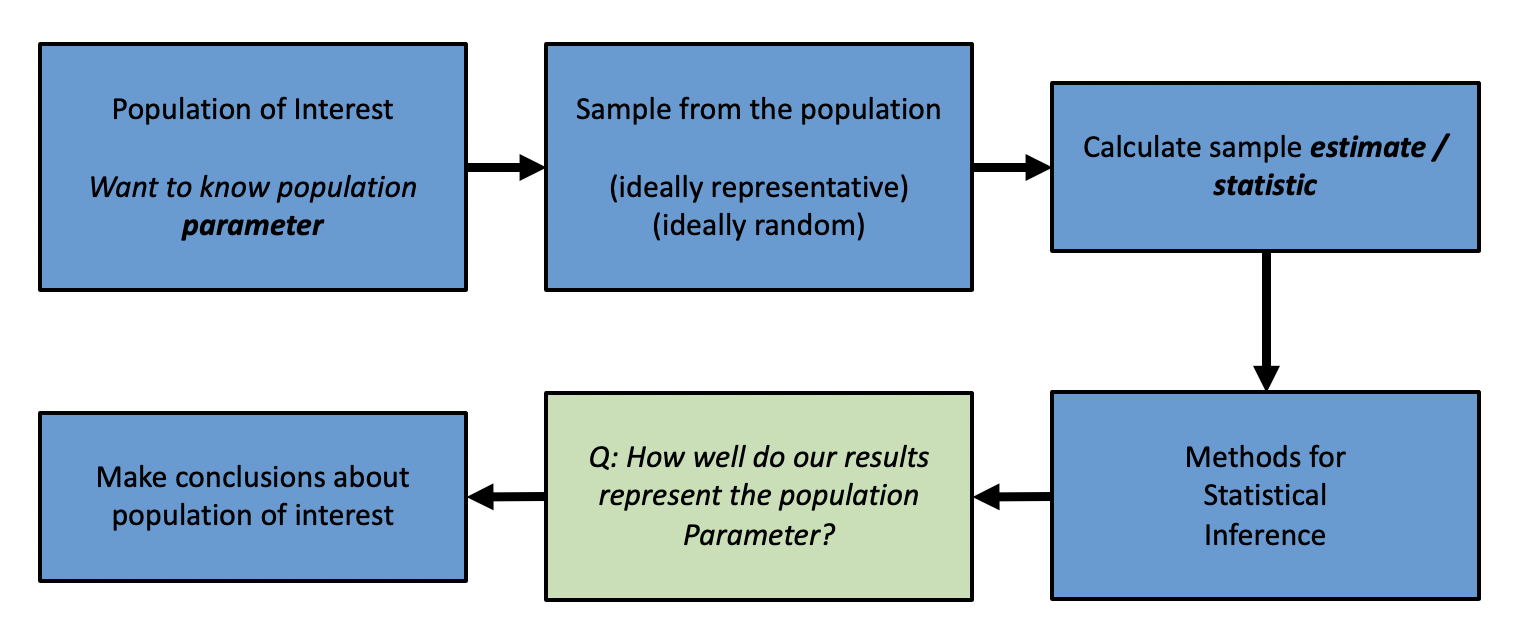
\includegraphics[scale=0.4]{statinference_workflow.png}
\end{frame}

\begin{frame}{Statistical Inference: Motivating example}

Consider our births dataset. We're interesting in knowing whether the First Steps program improves birth outcomes in King County.

\vspace{0.1cm}

\begin{itemize}
	\item \textbf{Scientific question:} what is the \textcolor{orange}{typical}  \textcolor{blue}{birth outcome} for an individual?

\end{itemize}

\end{frame}

\begin{frame}{Statistical Inference: Motivating example}

Consider our births dataset. We're interesting in knowing whether the First Steps program improves birth outcomes in King County.

\vspace{0.1cm}

\begin{itemize}
	\item \textbf{Scientific question:} what is the \textcolor{orange}{typical}  \textcolor{blue}{birth outcome} for an individual?
	\item \textbf{Statistical question:} what is the \textcolor{orange}{mean} \textcolor{blue}{birth weight} for an individual?
\end{itemize}

\end{frame}

\begin{frame}{Statistical Inference: Motivating example}

Consider our births dataset. We're interesting in knowing whether the First Steps program improves birth outcomes in King County.

\vspace{0.1cm}

\begin{itemize}
	\item \textbf{Scientific question:} what is the \textcolor{orange}{typical}  \textcolor{blue}{birth outcome} for an individual?
	\item \textbf{Statistical question:} what is the \textcolor{orange}{mean} \textcolor{blue}{birth weight} for an individual?
	\item \textbf{Population of interest:} all babies born in King County
\end{itemize}

\end{frame}

\begin{frame}{Statistical Inference: Motivating example}

Consider our births dataset. We're interesting in knowing whether the First Steps program improves birth outcomes in King County.

\vspace{0.1cm}

\begin{itemize}
	\item \textbf{Scientific question:} what is the \textcolor{orange}{typical}  \textcolor{blue}{birth outcome} for an individual?
	\item \textbf{Statistical question:} what is the \textcolor{orange}{mean} \textcolor{blue}{birth weight} for an individual?
	\item \textbf{Population of interest:} all babies born in King County
	\begin{itemize}
		\item \textbf{Parameter:} population mean
	\end{itemize}
\end{itemize}

\end{frame}

\begin{frame}{Statistical Inference: Motivating example}

Consider our births dataset. We're interesting in knowing whether the First Steps program improves birth outcomes in King County.

\vspace{0.1cm}

\begin{itemize}
	\item \textbf{Scientific question:} what is the \textcolor{orange}{typical}  \textcolor{blue}{birth outcome} for an individual?
	\item \textbf{Statistical question:} what is the \textcolor{orange}{mean} \textcolor{blue}{birth weight} for an individual?
	\item \textbf{Population of interest:} all babies born in King County
	\begin{itemize}
		\item \textbf{Parameter:} population mean
	\end{itemize}
	\item \textbf{Sample:} 2500 singleton births in King County in 2001
\end{itemize}

\end{frame}

\begin{frame}{Statistical Inference: Motivating example}

Consider our births dataset. We're interesting in knowing whether the First Steps program improves birth outcomes in King County.

\vspace{0.1cm}

\begin{itemize}
	\item \textbf{Scientific question:} what is the \textcolor{orange}{typical}  \textcolor{blue}{birth outcome} for an individual?
	\item \textbf{Statistical question:} what is the \textcolor{orange}{mean} \textcolor{blue}{birth weight} for an individual?
	\item \textbf{Population of interest:} all babies born in King County
	\begin{itemize}
		\item \textbf{Parameter:} population mean
	\end{itemize}
	\item \textbf{Sample:} 2500 singleton births in King County in 2001
	\begin{itemize}
		\item \textbf{Statistics/estimate:} sample mean (3414 grams)
	\end{itemize}
\end{itemize}

\end{frame}

\begin{frame}{Statistical Inference: Motivating example}

Consider our births dataset. We're interesting in knowing whether the First Steps program improves birth outcomes in King County.

\vspace{0.1cm}

\begin{itemize}
	\item \textbf{Scientific question:} what is the \textcolor{orange}{typical}  \textcolor{blue}{birth outcome} for an individual?
	\item \textbf{Statistical question:} what is the \textcolor{orange}{mean} \textcolor{blue}{birth weight} for an individual?
	\item \textbf{Population of interest:} all babies born in King County
	\begin{itemize}
		\item \textbf{Parameter:} population mean
	\end{itemize}
	\item \textbf{Sample:} 2500 singleton births in King County in 2001
	\begin{itemize}
		\item \textbf{Statistics/estimate:} sample mean (3414 grams)
	\end{itemize}
\end{itemize}

\vspace{0.1cm}

\small \textbf{Next step:} consider what conclusions can be drawn from our sample estimate about our population parameter. Was our sample representative? Are there implications (statistical, ethical) to generalizing our result to our population?

\end{frame}

\begin{frame}{Precision and Accuracy}
	
\vspace{-3 mm}
	
Using descriptive statistics, we can get sample estimates
\vspace{0.3cm}
\begin{itemize}
	\item e.g., the \textbf{mean} birthweight for singleton births in King County in 2001 was 3414 grams
\end{itemize}
\vspace{0.3cm}
We want to use these sample estimates to infer something about the population 
\vspace{0.3cm}

To assess how well these estimates represent the population of interest, we need to know how \textbf{accurate} and \textbf{precise} they are

\vspace{0.3cm}
\begin{itemize}
	\item Accuracy: are we estimating the right thing?
	\item Precision: how variable are our estimates?
\end{itemize}
\vspace{0.3cm}
\textbf{Just like we want to describe the center and spread of variables when we summarize our data, we also want to understand the center (accuracy) and spread (precision) of our estimates.}
\end{frame}

\begin{frame}[c]{Precision and Accuracy}
\centering 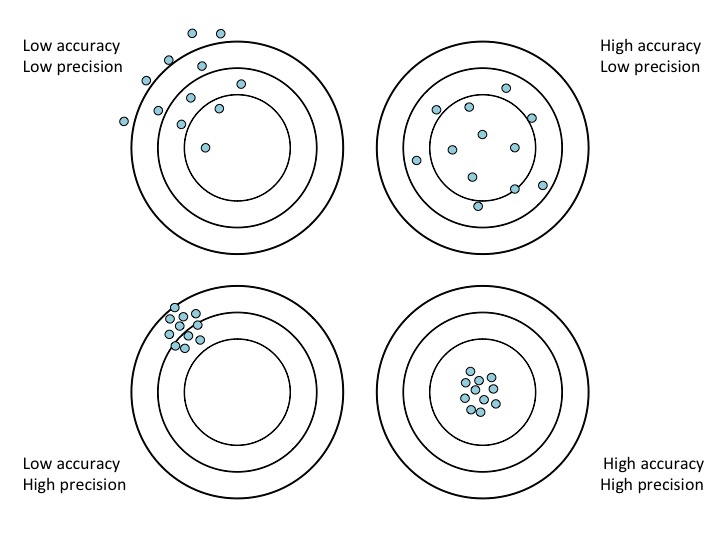
\includegraphics[scale=0.38]{accuracy.jpg}
\end{frame}

\begin{frame}{Precision, Accuracy, and Inference}
	
\vspace{-3 mm}
	
	
How do we know how precise or accurate our statistic is?

\vspace{0.1cm}

\begin{itemize}
	\item We need to know how our statistic (estimated from a sample) would vary in \textbf{repeated samples}
	\begin{itemize}
		\smallskip
		\item i.e., if we went out and collected another sample from this population, how different would the estimate be? And if we did this a third time, or a fourth time, etc.?
	\end{itemize}
\medskip
	\item Our statistics are \textbf{random}: the value you get will change depending on which sample you've ended up with
	\begin{itemize}
		\smallskip
		\item The \textbf{distribution} of a random quantity describes how that random quantity behaves
		\smallskip
		\item If we know the distribution of our statistic, the center tells us about the (possible${}^1$) accuracy and the spread tells us about the precision of our statistic
	\end{itemize}
\end{itemize}

\vspace{0.1cm}

\small ${}^1$ we only know how accurate our statistic is if we know the population parameter, but we can often judge if our statistics are very \textbf{inaccurate} based on whether our sample is representative of the population

\end{frame}

\subsection{Normal/$t$ distributions, Sampling distributions}

\begin{frame}{Probability distributions}
	
\vspace{-3 mm}	
	
	The \textcolor{blue}{distribution} of a random quantity tells you what values that quantity can take and how likely it is to take each of those values.
	\bigskip
	
	Discrete Variable
	\begin{figure}
	\centering 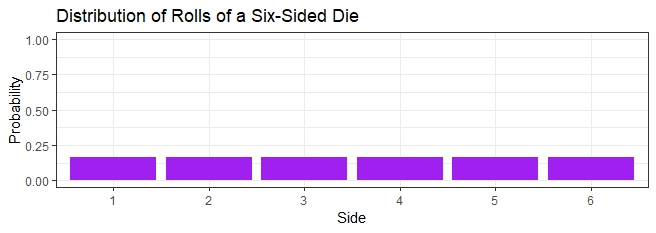
\includegraphics[scale=0.35]{discrete_dist}
	\end{figure}
	\smallskip
	
	Continuous Variable
\begin{figure}
	\centering 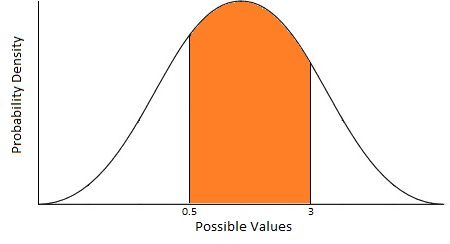
\includegraphics[scale=0.35]{Normal-density.jpg}
\end{figure}
\end{frame}


\begin{frame}{Probability distributions}
The \textcolor{blue}{distribution} of a random quantity tells you what values that quantity can take and how likely it is to take each of those values.

\begin{figure}
	\centering 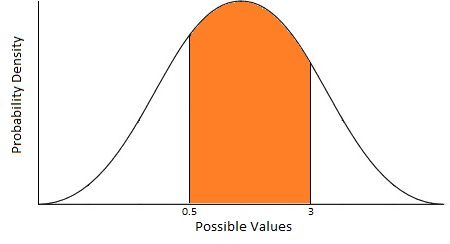
\includegraphics[scale=0.5]{Normal-density.jpg}
\end{figure}

\textcolor{blue}{Figure:} For continuous variables, \textcolor{orange}{Area under curve} = probability that our random quantity takes values between 0.5 and 3

\end{frame}

\begin{frame}{Probability distributions: normal distribution}

\begin{figure}
	\centering 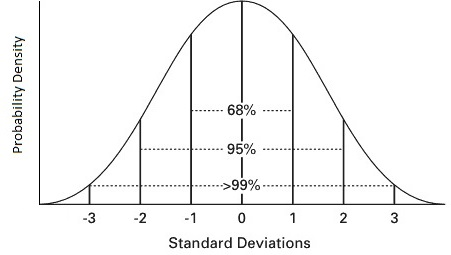
\includegraphics[scale=0.5]{Normal.jpg}
\end{figure}

\textcolor{blue}{Useful property:} if a random quantity is normally distributed $(~N(\mu, \sigma^2))$, then 95\% of the time that quantity will take values within 1.96 standard deviations $(\sigma)$ of its mean $(\mu)$

\vspace{0.3cm}

 \textcolor{blue}{Many of the random quantities we care about have a (approximately) normal distribution given a large enough sample size!} 

\end{frame}

\begin{frame}{Probability distributions: $t$ distribution}
\begin{figure}
	\centering 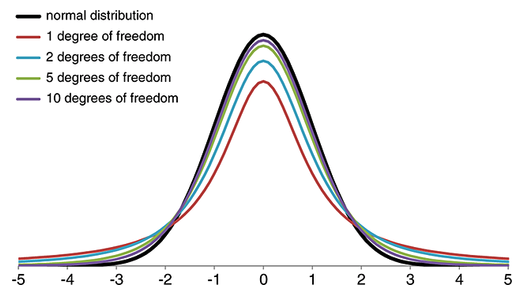
\includegraphics[scale=0.5]{tdistn.png}
\end{figure}

The $t$ distribution is similar to a normal distribution, but with heavier tails (so \textbf{less precision}). How close it is to a normal distribution depends on the \textbf{degrees of freedom}.

\end{frame}

\begin{frame}{Sampling distributions}

\textbf{Sampling distribution}: the distribution of an estimate/statistic

\vspace{0.3cm}

The \textcolor{orange}{Central Limit Theorem} tells us the sampling distribution of some statistics that we care about \textbf{for large samples}:
\medskip
\begin{itemize}
		\item \textbf{Mean:} \textcolor{blue}{the sampling distribution of the sample mean is approximately normal:} $\bar{X} \sim N(\mu, \sigma^2 / n)$
	\smallskip
	\begin{itemize}
		\item $\mu$ = population mean
		\smallskip
		\item $\sigma^2$ = population variance
		\smallskip
		\item $n$ = sample size
	\end{itemize}

\end{itemize}
\end{frame}

\begin{frame}{Sampling distributions}

\textbf{Sampling distribution}: the distribution of an estimate/statistic

\vspace{0.3cm}

The \textcolor{orange}{Central Limit Theorem} tells us the sampling distribution of some statistics that we care about \textbf{for large samples}:
\medskip
\begin{itemize}
	\item \textbf{Mean:} \textcolor{blue}{the sampling distribution of the sample mean is approximately normal:} $\bar{X} \sim N(\mu, \sigma^2 / n)$
	\smallskip
	\begin{itemize}
		\item $\mu$ = population mean
		\smallskip
		\item $\sigma^2$ = population variance
		\smallskip
		\item $n$ = sample size
	\end{itemize}
\medskip
	\item \textbf{Proportion:} \textcolor{blue}{the sampling distribution of the sample proportion is approximately normal:} $ \hat{p} \sim N(p, p(1-p)/n)$
	\begin{itemize}
		\smallskip
		\item $p$ = population proportion
		\smallskip
		\item $n$ = sample size / number of trials
	\end{itemize}
\end{itemize}
\end{frame}

\begin{frame}{Sampling distributions}

\vspace{-5 mm}

\textbf{Sampling distribution}: the distribution of an estimate/statistic

\vspace{0.3cm}

The \textcolor{orange}{Central Limit Theorem} tells us the sampling distribution of some statistics that we care about \textbf{for large samples}:
\medskip
\begin{itemize}
	\item \textbf{Mean:} \textcolor{blue}{the sampling distribution of the sample mean is approximately normal:} $\bar{X} \sim N(\mu, \sigma^2 / n)$
	\smallskip
	\begin{itemize}
		\item $\mu$ = population mean
		\smallskip
		\item $\sigma^2$ = population variance
		\smallskip
		\item $n$ = sample size
	\end{itemize}
	\medskip
	\item \textbf{Proportion:} \textcolor{blue}{the sampling distribution of the sample proportion is approximately normal:} $ \hat{p} \sim N(p, p(1-p)/n)$
	\begin{itemize}
		\smallskip
		\item $p$ = population proportion
		\smallskip
		\item $n$ = sample size / number of trials
	\end{itemize}
\medskip
Another statistic that we often care about $\frac{\bar{X} - \mu}{s} \sim t_{n - 1}$
\begin{itemize}
	\smallskip
	\item $s$ = sample standard deviation
\end{itemize}
\end{itemize}

\end{frame}

\subsection{Uncertainty: Standard errors, confidence intervals, p-values}

\begin{frame}{Standard error}
\textbf{Sampling distribution}: the distribution of an estimate/statistic
\medskip

\textbf{Standard error}: the standard deviation of an estimate/statistic

\vspace{0.3cm} 

Once we know the sampling distribution of our estimate, it's fairly straightforward to figure out how \textbf{precise} it is. 

\vspace{0.3cm}

\textcolor{violet}{POLLEV}: Suppose we have two estimates. The first has sampling distribution $N(2, 5)$ and the second has sampling distribution $N(2, 1)$. \textbf{Which of these estimates is more precise?}

\vspace{0.3cm}

(Hint: precision and variance are inversely related) 


\end{frame}

%\begin{frame}{Standard error}
%	\textbf{Sampling distribution}: the distribution of an estimate/statistic
%	\medskip
%	
%	\textbf{Standard error}: the standard deviation of an estimate/statistic
%	
%	\vspace{0.3cm} 
%	
%	Once we know the sampling distribution of our estimate, it's fairly straightforward to figure out how \textbf{precise} it is. 
%	
%	\vspace{0.3cm}
%	
%	\textcolor{violet}{POLLEV}: Suppose we have two estimates. The first has sampling distribution $N(2, 5)$ and the second has sampling distribution $N(2, 1)$. \textbf{Which of these estimates is more precise?}
%	
%	\vspace{0.3cm}
%	
%	(Hint: precision and variance are inversely related) 
%	
%	\vspace{0.3cm}
%	
%	\normalsize \textcolor{blue}{Answer:} We typically describe the precision of an estimate via its standard error. Estimates with \textbf{smaller} standard error are \textbf{more} precise. Therefore, the estimate with sampling distribution $N(2, 1)$ is more precise.
%\end{frame}

\begin{frame}{Standard error}
\textbf{Sampling distribution}: the distribution of an estimate/statistic
\medskip

\textbf{Standard error}: the standard deviation of an estimate/statistic

\vspace{0.3cm} 

The sampling distribution of the sample mean $\bar{X}$ is approximately normal: $\bar{X} \sim N(\mu, \sigma^2/n)$

\vspace{0.3cm}

\textcolor{blue}{Question}: What is the standard error? \pause

\vspace{0.3cm}

\textcolor{blue}{Answer}: The standard deviation of the sample mean, which is $\sqrt{\sigma^2/n}$.
\end{frame}

\begin{frame}{Standard error}
\textbf{Sampling distribution}: the distribution of an estimate/statistic
\medskip

\textbf{Standard error}: the standard deviation of an estimate/statistic

\vspace{0.3cm} 

The sampling distribution of the sample proportion $\hat{p}$ is approximately normal: $\hat{p} \sim N(p, p(1-p)/n)$

\vspace{0.3cm}

\textcolor{blue}{Question}: What is the standard error? \pause

\vspace{0.3cm}

\textcolor{blue}{Answer}: The standard deviation of the sample proportion, which is $\sqrt{p(1-p)/n}$.
\end{frame}

\begin{frame}{Reporting uncertainty: Motivating example}
Recall our motivating example for statistical inference:

\vspace{0.3cm}

We're interesting in knowing whether the First Steps program improves birth outcomes in King County.

\vspace{0.1cm}

\begin{itemize}
	\item \textbf{Scientific question:} what is the \textcolor{orange}{typical}  \textcolor{blue}{birth outcome} for an individual?
	\item \textbf{Statistical question:} what is the \textcolor{orange}{mean} \textcolor{blue}{birth weight} for an individual?
	\item \textbf{Population of interest:} all babies born in King County
	\begin{itemize}
		\item \textbf{Parameter:} population mean
	\end{itemize}
	\item \textbf{Sample:} 2500 singleton births in King County in 2001
	\begin{itemize}
		\item \textbf{Statistic/estimate:} sample mean (3414 grams)
	\end{itemize}
\end{itemize}

\end{frame}

\begin{frame}{Reporting uncertainty: Motivating example}
	
\vspace{-3 mm}
	
We can convert this outline into general steps for a statistical inference procedure:

\vspace{0.3cm}

\begin{enumerate}
	\item Start with a \textbf{scientific question:} what is the typical birth outcome for an individual?
	\item Convert to a \textbf{statistical question:} what is the mean birth weight for an individual?
	\begin{itemize}
		\item Identify the \textbf{population} (all babies born in King County) and \textbf{parameter} (population mean) of interest
	\end{itemize}
	\item Take a \textbf{sample} from the population: 2500 singleton births in King County in 2001
	\item Perform \textbf{statistical inference}:
	\begin{itemize}
		\item Calculate the corresponding \textbf{statistic} (sample mean): 3414 grams
		\item Quantify the uncertainty in your statistic
	\end{itemize}
	\item Make conclusions about your original scientific and statistical questions
\end{enumerate}
\end{frame}

\begin{frame}{Reporting uncertainty: Motivating example}

\vspace{-3 mm}

We can convert this outline into general steps for a statistical inference procedure:

\vspace{0.3cm}

\begin{enumerate}
	\item Start with a \textbf{scientific question:} what is the typical birth outcome for an individual?
	\item Convert to a \textbf{statistical question:} what is the mean birth weight for an individual?
	\begin{itemize}
		\item Identify the \textbf{population} (all babies born in King County) and \textbf{parameter} (population mean) of interest
	\end{itemize}
	\item Take a \textbf{sample} from the population: 2500 singleton births in King County in 2001
	\item Perform \textbf{statistical inference}:
	\begin{itemize}
		\item Calculate the corresponding \textbf{statistic} (sample mean): 3414 grams
		\item \textcolor{blue}{Quantify the uncertainty in your statistic $\leftarrow$ \textbf{two options}}
	\end{itemize}
	\item Make conclusions about your original scientific and statistical questions
\end{enumerate}
\end{frame}

\begin{frame}{Reporting uncertainty: Motivating example}
We've calculated our statistic: average birthweight = 3414 grams

\vspace{0.3cm}

Now we need to quantify our uncertainty in this estimate.

\vspace{0.3cm}

\textcolor{blue}{Option 1:} use the standard error
\smallskip

\textbf{We estimate that the average birthweight is 3414 grams, with standard error 0.224.}

\vspace{0.3cm}

\textcolor{blue}{Option 2:} use a 95\% confidence interval (est $\pm 1.96 \times SE$)
\smallskip

\textbf{We estimate that the average birthweight is 3414 grams. Based on a 95\% confidence interval, this observed average would not be considered unusual if the true average birthweight were between 3413.6 and  3414.5 grams.}
\medskip

\textbf{We estimate that the average birthweight is 3414 grams, with a 95\% confidence interval of (3413.6, 3414.5) grams.}

\end{frame}

%\begin{frame}{Confidence Intervals}
%What does a 95\% confidence interval really mean, and how do we correctly interpret it?
%
%\vspace{0.3cm}
%
%The procedure of creating a 95\% confidence interval (est $\pm 1.96 \times SE$) gives us a range of values based on our sample.
%
%\centering 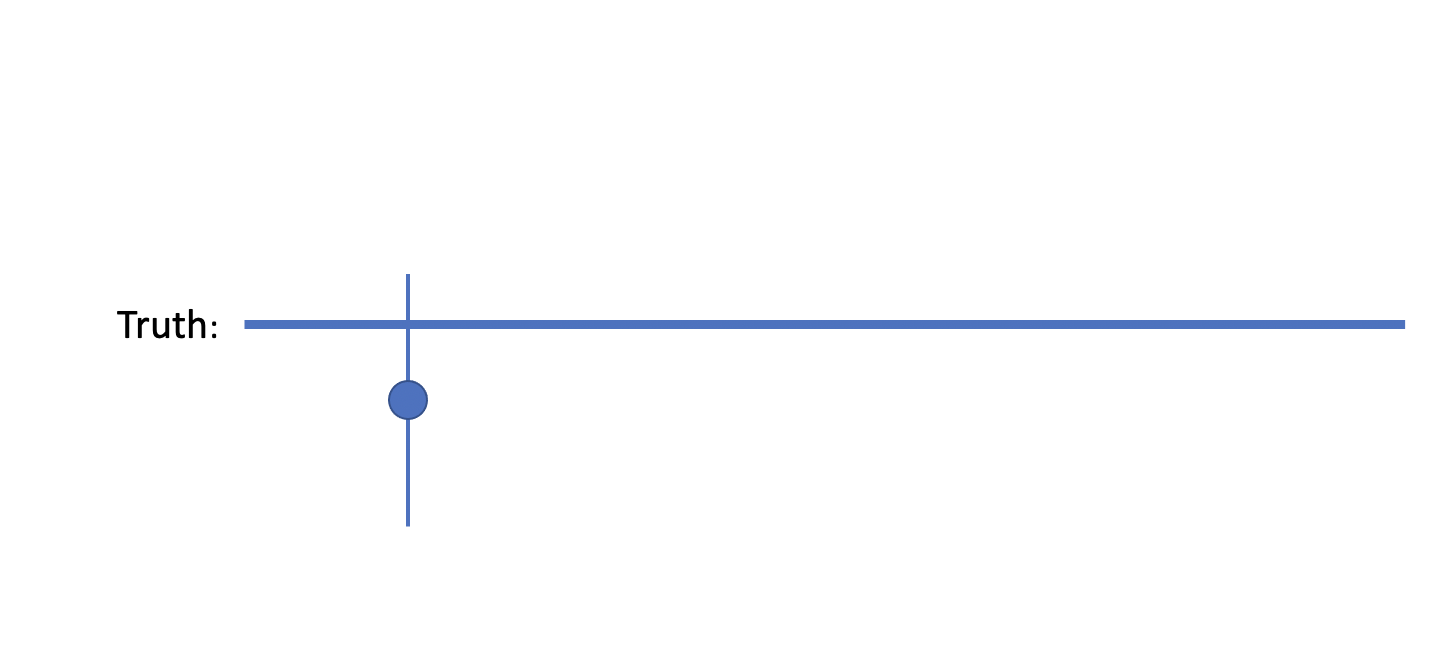
\includegraphics[scale=0.4]{ci1.png}
%
%\end{frame}
%
%\begin{frame}{Confidence Intervals}
%What does a 95\% confidence interval really mean, and how do we correctly interpret it?
%
%\vspace{0.3cm}
%
%The procedure of creating a 95\% confidence interval (est $\pm 1.96 \times SE$) gives us a range of values based on our sample.
%
%\centering 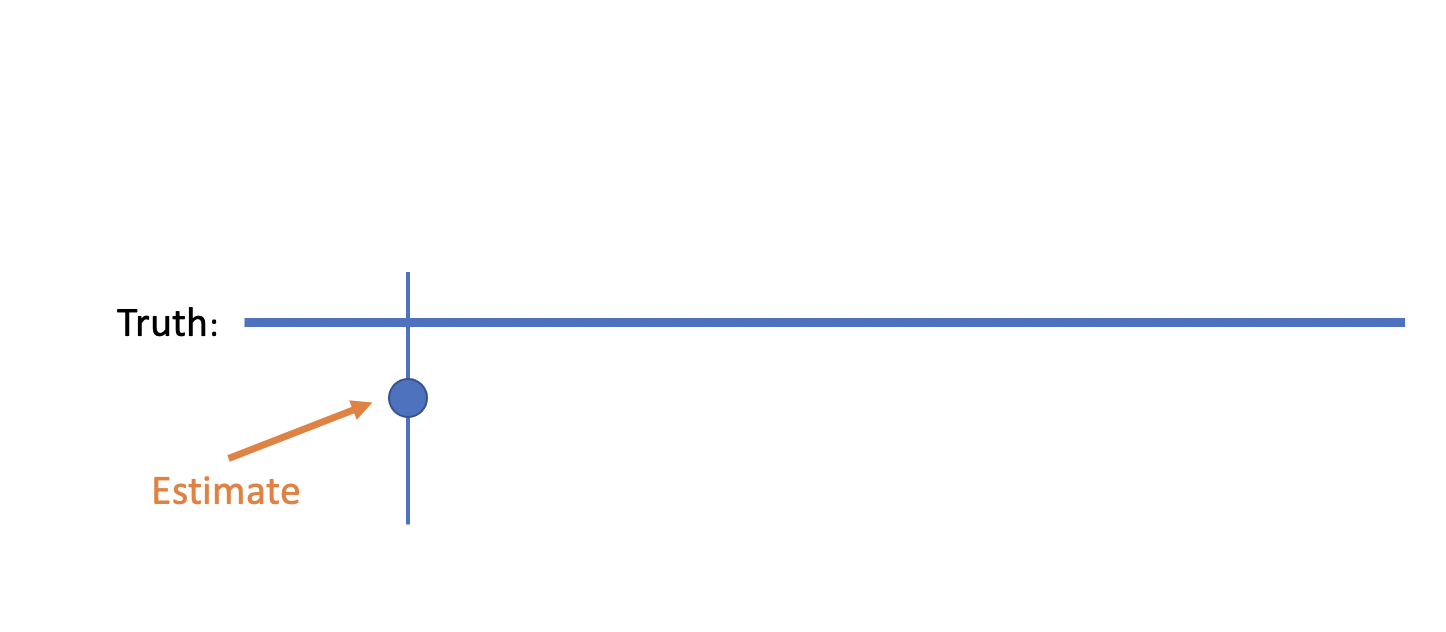
\includegraphics[scale=0.4]{ci2.png}
%
%\end{frame}

\begin{frame}{Confidence Intervals}
What does a 95\% confidence interval really mean, and how do we correctly interpret it?

\vspace{0.3cm}

The procedure of creating a 95\% confidence interval (est $\pm 1.96 \times SE$) gives us a range of values based on our sample.

\centering 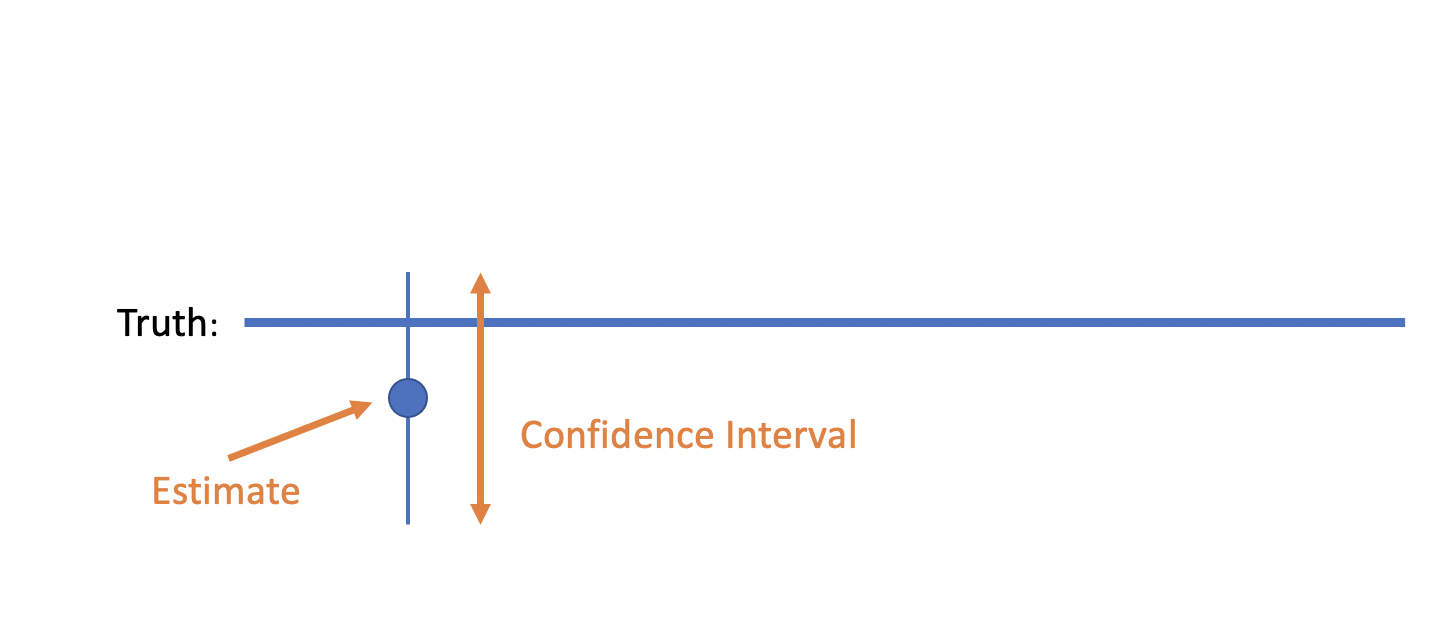
\includegraphics[scale=0.4]{ci3.png}

\end{frame}

\begin{frame}{Confidence Intervals}
The particular range of values that we get depends on the sample data, and will change if we go collect a second sample \dots

\centering 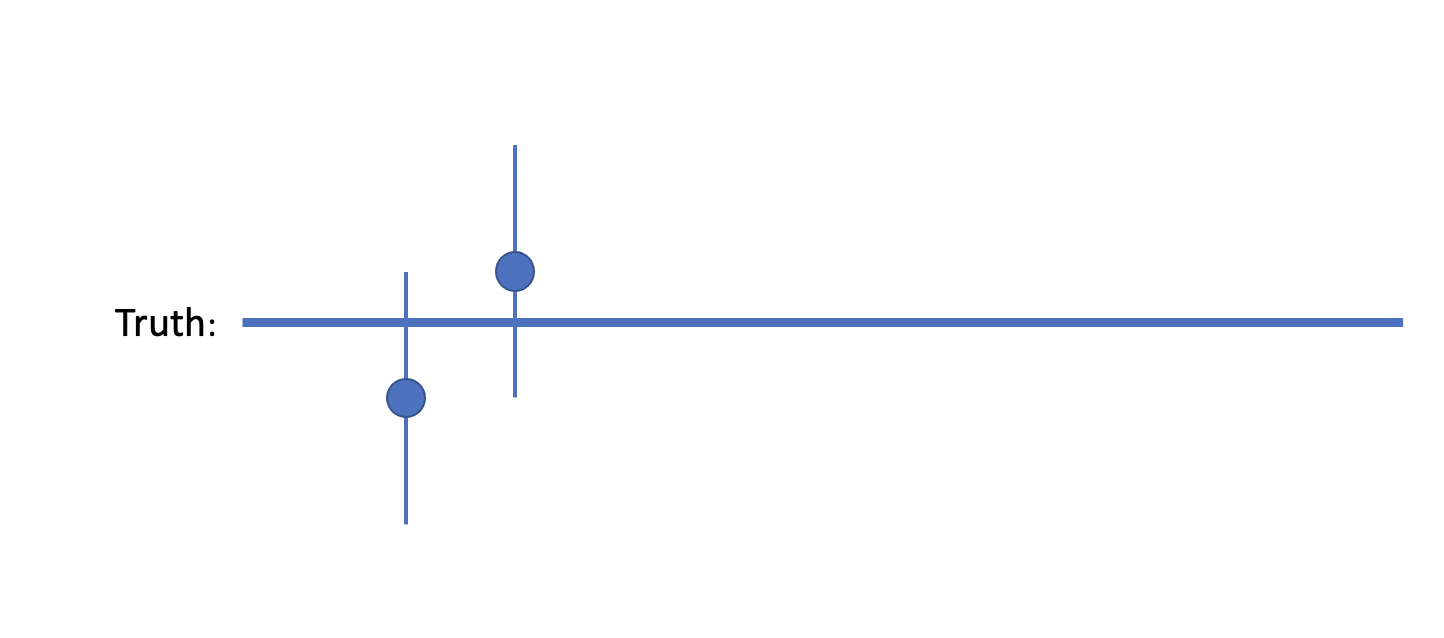
\includegraphics[scale=0.4]{ci4.png}

\end{frame}

\begin{frame}{Confidence Intervals}
\dots or a third sample \dots

\centering 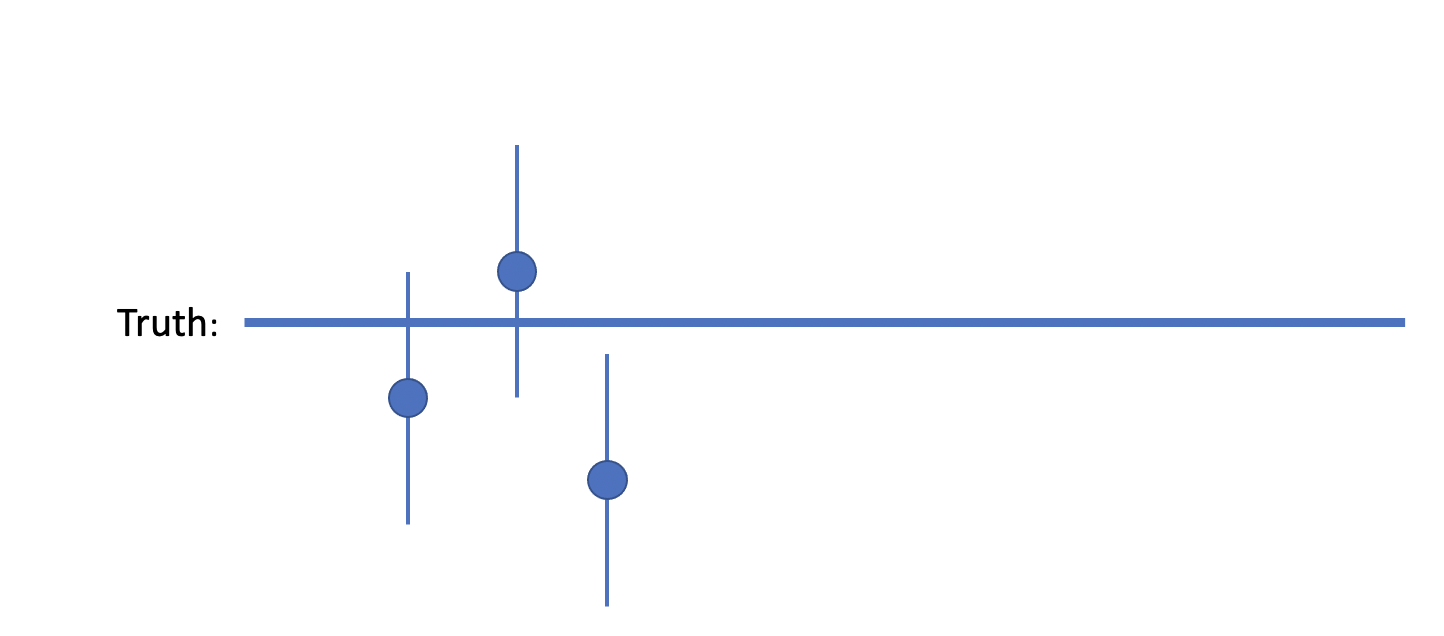
\includegraphics[scale=0.4]{ci5.png}

\end{frame}

\begin{frame}{Confidence Intervals}
Over (hypothetical) \textbf{repeated sampling}, 95\% \textbf{of these intervals} will cover the truth.

\centering 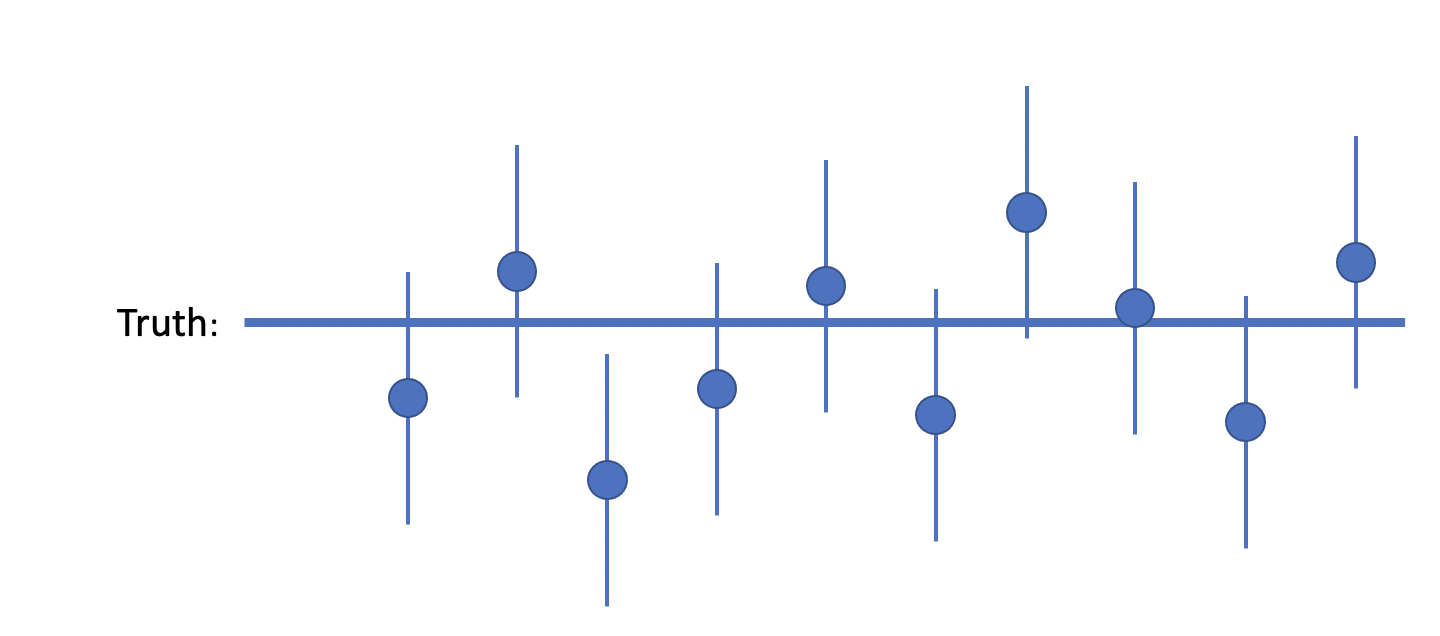
\includegraphics[scale=0.4]{ci6.png}

\end{frame}

\begin{frame}{Confidence Intervals}

\begin{figure}
\centering 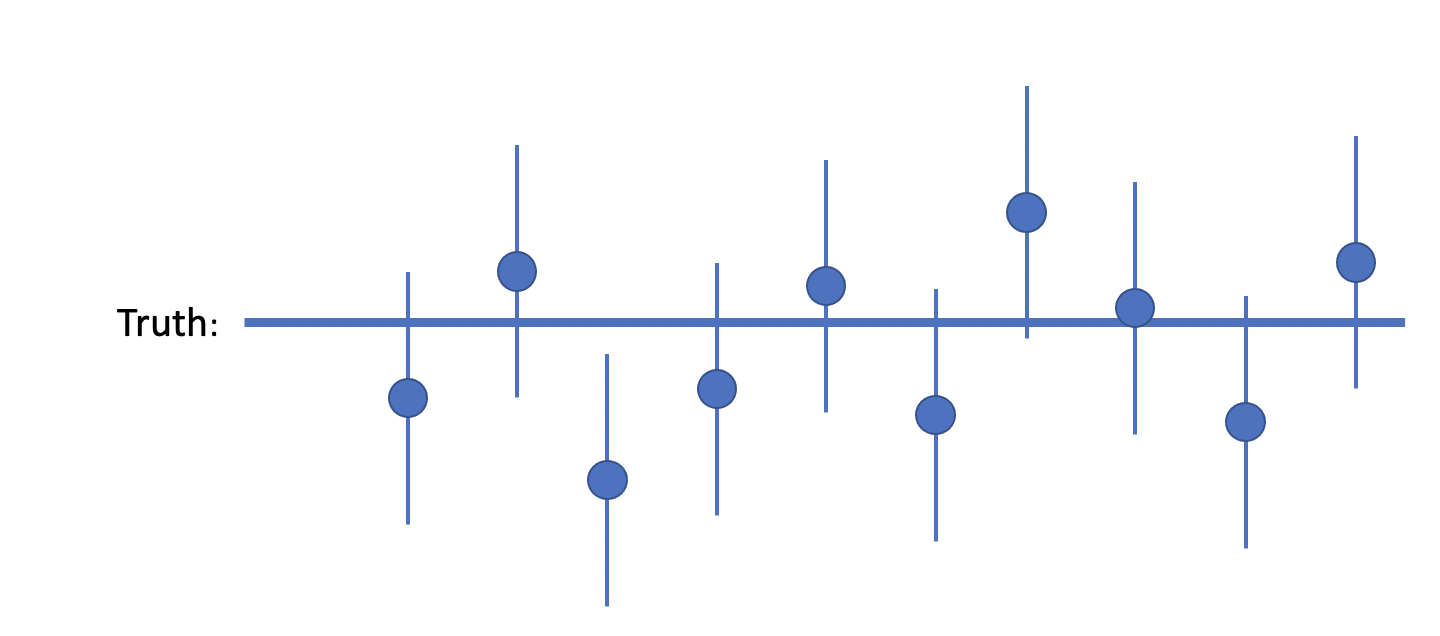
\includegraphics[scale=0.4]{ci6.png}
\end{figure}


\textcolor{blue}{Important:} it is not \textbf{our interval} that contains the truth 95\% of the time. Our interval either contains the truth, or it doesn't (as the image above shows). It is the \textbf{procedure} of computing confidence intervals over \textbf{repeated sampling} that gives us 95\% coverage of the truth.

\end{frame}

\begin{frame}{\textcolor{violet}{POLLEV}: Interpreting Confidence Intervals}
95\% CI for mean birthweight in grams is: (3413.6, 3414.5)

\vspace{0.3cm}

Which of these are correct interpretations?

\vspace{0.3cm}

\begin{enumerate}
	\item 95\% of children have birthweights between 3413.6 and 3414.5 grams.
	\medskip
	\item Our observed sample mean of 3414 grams would not be considered unusual if the true population mean birthweight were between 3413.6 and 3414.5 grams.
	\medskip
	\item There is a 95\% chance that the true population mean birthweight is between 3413.6 and 3414.5 grams.
\end{enumerate}
\end{frame}

%\begin{frame}{\textcolor{violet}{POLLEV}: Interpreting Confidence Intervals}
%95\% CI for mean birthweight in grams is: (3413.6, 3414.5)
%
%\vspace{0.3cm}
%
%Which of these are correct interpretations?
%
%\vspace{0.3cm}
%
%\begin{enumerate}
%	\item 95\% of children have birthweights between 3413.6 and 3414.5 grams.
%	\medskip
%	\item \textcolor{blue}{Our observed sample mean of 3414 grams would not be considered unusual if the true population mean birthweight were between 3413.6 and 3414.5 grams.}
%	\medskip
%	\item There is a 95\% chance that the true population mean birthweight is between 3413.6 and 3414.5 grams.*
%\end{enumerate}
%
%\small *this is a common mistake, and is \textbf{not} the correct interpretation of a confidence interval!
%
%\end{frame}

\begin{frame}{Interpreting Confidence Intervals: How-to}
Confidence intervals should always be interpreted \textbf{in context}.

\vspace{0.3cm}

When interpreting confidence intervals, it may be useful to have a ``word formula" to refer back to. An example of this is:

\vspace{0.3cm}

Our observed sample \textcolor{orange}{estimate} of \_\_\_ \textcolor{orange}{units} would not be considered unusual if the true population \textcolor{orange}{parameter} were between \_\_\_ and \_\_\_ \textcolor{orange}{units}.

\end{frame}

\begin{frame}{Interpreting Confidence Intervals: How-to}
Confidence intervals should always be interpreted \textbf{in context}.

\vspace{0.3cm}

When interpreting confidence intervals, it may be useful to have a ``word formula" to refer back to. An example of this is:

\vspace{0.3cm}

Our observed sample \textcolor{orange}{estimate} of \_\_\_ \textcolor{orange}{units} would not be considered unusual if the true population \textcolor{orange}{parameter} were between \_\_\_ and \_\_\_ \textcolor{orange}{units}.

\vspace{0.3cm}

Replacing the \textcolor{orange}{orange} words and filling in the blanks for our example, we get:

\vspace{0.3cm}

Our observed sample \textcolor{orange}{mean} of 3414 \textcolor{orange}{grams} would not be considered unusual if the true population \textcolor{orange}{mean birthweight} were between 3413.6 and 3414.5 \textcolor{orange}{grams}.

\end{frame}

\begin{frame}{Statistical Inference: New Example}

\begin{enumerate}
	\item \textbf{Scientific question:} do birth parents in King County who participated in First Steps (FS) have \textcolor{orange}{different} \textcolor{blue}{birth outcomes}?
\end{enumerate}

\end{frame}

\begin{frame}{Statistical Inference: New Example}

\begin{enumerate}
	\item \textbf{Scientific question:} do birth parents in King County who participated in First Steps (FS) have \textcolor{orange}{different} \textcolor{blue}{birth outcomes}?
	\item \textbf{Statistical question:} is there a \textcolor{orange}{difference in average} \textcolor{blue}{birthweight} between birth parents in FS and those not in the program?
\end{enumerate}

\end{frame}

\begin{frame}{Statistical Inference: New Example}

\begin{enumerate}
	\item \textbf{Scientific question:} do birth parents in King County who participated in First Steps (FS) have \textcolor{orange}{different} \textcolor{blue}{birth outcomes}?
	\item \textbf{Statistical question:} is there a \textcolor{orange}{difference in average} \textcolor{blue}{birthweight} between birth parents in FS and those not in the program?
	\begin{itemize}
		\item \textbf{Population} = all babies born in King County, \textbf{parameter} = difference in population means (between babies born to parents in FS vs. not)
	\end{itemize}
\end{enumerate}

\end{frame}

\begin{frame}{Statistical Inference: New Example}

\begin{enumerate}
	\item \textbf{Scientific question:} do birth parents in King County who participated in First Steps (FS) have \textcolor{orange}{different} \textcolor{blue}{birth outcomes}?
	\item \textbf{Statistical question:} is there a \textcolor{orange}{difference in average} \textcolor{blue}{birthweight} between birth parents in FS and those not in the program?
	\begin{itemize}
		\item \textbf{Population} = all babies born in King County, \textbf{parameter} = difference in population means (between babies born to parents in FS vs. not)
	\end{itemize}
	\item Take a \textbf{sample} from the population: 2500 singleton births in King County in 2001
\end{enumerate}

\end{frame}

\begin{frame}{Statistical Inference: New Example}

\begin{enumerate}
	\item \textbf{Scientific question:} do birth parents in King County who participated in First Steps (FS) have \textcolor{orange}{different} \textcolor{blue}{birth outcomes}?
	\item \textbf{Statistical question:} is there a \textcolor{orange}{difference in average} \textcolor{blue}{birthweight} between birth parents in FS and those not in the program?
	\begin{itemize}
		\item \textbf{Population} = all babies born in King County, \textbf{parameter} = difference in population means (between babies born to parents in FS vs. not)
	\end{itemize}
	\item Take a \textbf{sample} from the population: 2500 singleton births in King County in 2001
	\item Perform \textbf{statistical inference}:
	\begin{itemize}
		\item Calculate the corresponding \textbf{statistic} (difference in sample means between FS vs. not)
		\item Quantify the uncertainty in our statistic
		\item Perform a hypothesis test
	\end{itemize}
\end{enumerate}

\end{frame}

\begin{frame}{Statistical Inference: New Example}

\begin{enumerate}
	\item \textbf{Scientific question:} do birth parents in King County who participated in First Steps (FS) have \textcolor{orange}{different} \textcolor{blue}{birth outcomes}?
	\item \textbf{Statistical question:} is there a \textcolor{orange}{difference in average} \textcolor{blue}{birthweight} between birth parents in FS and those not in the program?
	\begin{itemize}
		\item \textbf{Population} = all babies born in King County, \textbf{parameter} = difference in population means (between babies born to parents in FS vs. not)
	\end{itemize}
	\item Take a \textbf{sample} from the population: 2500 singleton births in King County in 2001
	\item Perform \textbf{statistical inference}:
	\begin{itemize}
		\item Calculate the corresponding \textbf{statistic} (difference in sample means between FS vs. not)
		\item Quantify the uncertainty in our statistic
		\item Perform a hypothesis test
	\end{itemize}
	\item Make conclusions in context of original questions
\end{enumerate}

\end{frame}

\begin{frame}{Statistical Inference: New Example}
To perform statistical inference, we need:

\vspace{0.3cm}

A \textbf{statistic}: difference in average birthweight \textbf{in our sample} between babies born to parents in FS vs. not in FS 

\vspace{0.3cm}

\textbf{Uncertainty} in our statistic: 95\% confidence interval for difference in average birthweight

\vspace{0.3cm}

To perform a \textbf{hypothesis test:}
\smallskip
\begin{itemize}
	\item \textbf{Null and alternative hypotheses}:
	\begin{itemize}
		\item $H_0$: $\mu_{\text{FS}} - \mu_{\text{no FS}} = 0$
		\item $H_1$: $\mu_{\text{FS}} - \mu_{\text{no FS}} \neq 0$
	\end{itemize}
\smallskip
	\item \textbf{Choice of test}: two-sample t-test (unequal variances)
	\begin{itemize}
		\item Test if the averages in two independent groups are equal
		\item We will not assume variance in birthweight is the same in babies born to parents in FS vs. not in FS
	\end{itemize}
\end{itemize}


\end{frame}

\begin{frame}[fragile=singleslide]{Statistical Inference: New Example}

\vspace{-5 mm}

We can conduct a two-sample t-test to answer this question in \texttt{R}:



\small
\begin{verbatim}t.test(data = births, bwt ~ firstep, var.equal = FALSE)\end{verbatim}
\smallskip

\begin{verbatim}
Welch Two Sample t-test
\end{verbatim}
\begin{verbatim}
data:  bwt by firstep
\end{verbatim}
\begin{verbatim}
t = 2.0239, df = 533.75, p-value = 0.04347
\end{verbatim}
\begin{verbatim}
alternative hypothesis: true difference in means between group 0 
and group 1 is not equal to 0
\end{verbatim}
\begin{verbatim}
95 percent confidence interval:
1.946111 130.415827
\end{verbatim}
\begin{verbatim}
sample estimates:
mean in group 0 mean in group 1 
3424.687        3358.506
\end{verbatim}

\end{frame}


\begin{frame}[fragile=singleslide]{Statistical Inference: New Example}
	
	\vspace{-5 mm}
	
	We can conduct a two-sample t-test to answer this question in \texttt{R}:
	
	

\small
\begin{verbatim}t.test(data = births, bwt ~ firstep, var.equal = FALSE)\end{verbatim}
	\smallskip
	
	\begin{verbatim}
	Welch Two Sample t-test
	\end{verbatim}
	\begin{verbatim}
	data:  bwt by firstep
	\end{verbatim}
	\begin{verbatim}
	t = 2.0239, df = 533.75, p-value = 0.04347
	\end{verbatim}
	\begin{verbatim}
	alternative hypothesis: true difference in means between group 0 
	and group 1 is not equal to 0
	\end{verbatim}
	\begin{verbatim}
	95 percent confidence interval:
	1.946111 130.415827
	\end{verbatim}
	\begin{verbatim}
	sample estimates:
	mean in group 0 mean in group 1 
	3424.687        3358.506
	\end{verbatim}

\begin{itemize}
	\item The observed difference in means is $3424.687-  3358.506 \approx 66$ grams, with group $0$ having the higher mean
	\item The 95\% confidence interval for the difference is $(1.95, 130.42)$
	\item The p-value corresponding to this test is $0.04$
\end{itemize}

\end{frame}


\begin{frame}{Interpreting p-values}
\textbf{Definition:} a \textbf{p-value} is the probability of obtaining a test statistic \textbf{as or more extreme} than the observed test statistic (computed from your data) under the null hypothesis

\begin{itemize}
	\item[] \textcolor{red}{Not} the probability that the alternative hypothesis is true! 
\end{itemize}

\vspace{0.3cm} 

(A less official definition): a \textbf{p-value} is a number between 0 and 1 that quantifies the statistical strength of your evidence against the null hypothesis

\vspace{0.3cm}

Values closer to 0 correspond to stronger evidence
\begin{itemize}
	\item Reject $H_0$ if p-value ($p$) is smaller than some pre-specified threshold $\alpha$ (usually 0.05)
	\item If $p < \alpha$ we declare``statistical significance" and reject $H_0$
	\item \textcolor{red}{We never accept the null hypothesis:} our options are to ``reject $H_0$" or ``fail to reject $H_0$"
\end{itemize}

\end{frame}

\begin{frame}{Statistical Inference: New Example}
Interpreting our results:

\vspace{0.3cm}

\begin{itemize}
	\item \textbf{Statistic:} We estimate that the difference in mean birthweight between babies born to birth parents in FS vs. those not in FS is 66 grams (with those not in FS having higher mean birthweight).
\end{itemize}

\end{frame}

\begin{frame}{Statistical Inference: New Example}
Interpreting our results:

\vspace{0.3cm}

\begin{itemize}
	\item \textbf{Statistic:} We estimate that the difference in mean birthweight between babies born to birth parents in FS vs. those not in FS is 66 grams (with those not in FS having higher mean birthweight).
	\item \textbf{Uncertainty:} Based on a 95\% confidence interval, this observed difference would not be surprising if the true difference were between 1.95 and 130.42 grams.
\end{itemize}

\end{frame}

\begin{frame}{Statistical Inference: New Example}
Interpreting our results:

\vspace{0.3cm}

\begin{itemize}
	\item \textbf{Statistic:} We estimate that the difference in mean birthweight between babies born to birth parents in FS vs. those not in FS is 66 grams (with those not in FS having higher mean birthweight).
	\item \textbf{Uncertainty:} Based on a 95\% confidence interval, this observed difference would not be surprising if the true difference were between 1.95 and 130.42 grams.
	\item \textbf{Hypothesis test p-value:} These data provide statistically significant evidence that the difference in mean birthweight between groups is different from zero ($p < 0.05$).
\end{itemize}

\end{frame}

\begin{frame}{Statistical Inference: New Example}
Interpreting our results:

\vspace{0.3cm}

\begin{itemize}
	\item \textbf{Statistic:} We estimate that the difference in mean birthweight between babies born to birth parents in FS vs. those not in FS is 66 grams (with those not in FS having higher mean birthweight).
	\item \textbf{Uncertainty:} Based on a 95\% confidence interval, this observed difference would not be surprising if the true difference were between 1.95 and 130.42 grams.
	\item \textbf{Hypothesis test p-value:} These data provide statistically significant evidence that the difference in mean birthweight between groups is different from zero ($p < 0.05$).
	\item \textbf{Conclusion:} These data provide statistically significant evidence to suggest that First Steps participation is associated with birthweight in children.
\end{itemize}

\end{frame}

\begin{frame}{Statistical Inference: New Example}
Interpreting our results:

\vspace{0.3cm}

\begin{itemize}
	\item \textbf{Statistic:} We estimate that the difference in mean birthweight between babies born to birth parents in FS vs. those not in FS is 66 grams (with those not in FS having higher mean birthweight).
	\item \textbf{Uncertainty:} Based on a 95\% confidence interval, this observed difference would not be surprising if the true difference were between 1.95 and 130.42 grams.
	\item \textbf{Hypothesis test p-value:} These data provide statistically significant evidence that the difference in mean birthweight between groups is different from zero ($p < 0.05$).
	\item \textbf{Conclusion:} These data provide statistically significant evidence to suggest that First Steps participation is associated with birthweight in children.
\end{itemize}

\vspace{0.1cm}

\textcolor{blue}{Always give 4 numbers:} point estimate, confidence interval (lower, upper), p-value (even when not significant!)

\end{frame}

\begin{frame}[c]
\centering \huge Any Questions?
\end{frame}

\end{document}